\documentclass{book}
\usepackage{commeunjeustyle}
\begin{document}
\chapter*{Probabilité finie}

%\dominitoc
La théorie des probabilités fournit des modèles mathématiques permettant
l'étude d'expériences dont le résultat ne peut être prévu avec  
certitude.

\begin{center}

\begin{tabular}{| p{6.5cm}| p{6.5cm} |p{1.7cm} |}
\hline
Expérience & Univers  $\Omega$ (ensemble des issues) & cardinal\\
\hline \hline 
Lancer d'un dé & Un entier $k\in\Intf{1}{6}$& fini \\
\hline
Prélèvement de n objets en sortie d'une chaîne de production dans l'échantillon & Nombre d'objets défectueux, $k\in\Intf{0}{n}$& fini\\
\hline
Questionnaire à 100 questions  binaires & Suite $\omega$ de 100 réponses $\omega\in\{0,1\}^{100}$& fini\\
\hline
Lancer d'une pièce jusqu'à la première obtention de pile & Un entier $k \in \mathbb{N}$ : le temps d'attente du premier succès&dénombrable\\
\hline
Temps d'attente pour une hotline  & un temps $\omega\in [0,+\infty[$&continue\\
\hline
Mouvement d'un grain de pollen dans un liquide & Une fonction continue : la trajectoire $f:\mathbb{R}^+\to\mathbb{R}^2$&continue  \\
\hline
Mouvement d'un cours boursier & Une fonction continue : $f:\mathbb{R}^+\to\mathbb{R}$&continue\\
\hline
 \end{tabular}
\end{center}
Bien que le résultat précis de chacune de ces expériences soit imprévisible,
l'observation et l'intuition nous amènent à penser que ces phénomènes
obéissent à certaines lois. Par exemple si on jette 6000 fois le dé, on s'attend
à ce que le nombre d'apparitions de la face « 3 » soit voisin de 1000. Si on
met en service 100 ampoules, leurs durées de vie observées seront concentrées
autour d'une certaine valeur moyenne.\\
La \defi{théorie des probabilités} modélise l'expérience aléatoire dans un cadre formel en quantifiant le sentiment d'incertitude vis-à-vis d'un événement. La \defi{statistique} permet de confronter les modèles probabilistes avec la réalité observée afin de les valider ou de les invalider. Par
exemple si quelqu'un a 60 bonnes réponses sur 100 au questionnaire, est-il
légitime de considérer qu'il a « mieux fait » que le hasard ?\\
Dans le cadre de cours, on limite l'univers à un ensemble \defi{fini}, c'est à dire que l'on peut effectuer une énumération finie des issues de l'expérience aléatoire.    
 
\section{Modélisation probabilistes pour un univers fini}
\subsection{Axiomes des probabilité. Premières propriétés}
\begin{Definition}[Univers]
Un \defi{univers}, noté $\Omega$, est l'ensemble de toutes les \defi{issues} (résultats) qui peuvent être obtenues au cours d'une expérience aléatoire. Une issue est noté $\omega$. Dans toute la suite de cours, on suppose que $\Omega$ est fini. 
\end{Definition}
\begin{Exemple}[Lancer de un dé]
Pour l'expérience aléatoire du lancer d'un dé, l'univers est $\Omega=\{1,2,3,4,5,6\}$. 
\end{Exemple}


\begin{Definition}[Événement]
Un \defi{événement} est une partie de l'univers. Un événement est dit \defi{élémentaire} si il contient une unique issue.
\end{Definition} 
\begin{Exemple}
Pour l'expérience aléatoire du lancer d'un dé, l'événement $A$="Obtenir un chiffre pair" est l'ensemble $\{2,4,6\}$. Il n'est pas élémentaire car il est composé de trois issues : 2, 4 et 6.
\end{Exemple}

\begin{Definition}[Notions et opérations]
Les notions et opérations que l'on définit sur les événements correspondent aux notions et opérations  que l'on définit sur les ensembles.
\begin{center}
\begin{tabular}{|p{1.4cm}|l|p{3cm}|l|}
\hline
Notations&	Vocabulaire ensembliste&	Vocabulaire probabiliste& Diagramme de Venn	\\
\hline
\hline
$\emptyset$&	ensemble vide&	événement impossible&	\\
\hline
$\Omega$&	ensemble plein&	événement certain& 
\begin{tikzpicture}[scale=0.5]\fill[color=cyan](-4,-1) rectangle (4,4);\node[above right] at (-4,-1) {$\Omega$};\end{tikzpicture}	\\
\hline
$\omega$&	élément de $\Omega$& issue&\begin{tikzpicture}[scale=0.5]\draw (-4,-1) rectangle (4,4);\node[above right] at (-4,-1) {$\Omega$};\node[above right] at (0,0) {$\omega$};\node at (0,0) {$\bullet$};\end{tikzpicture}	\\
\hline
$\{\omega\}$&	singleton&	événement élémentaire&	\\
\hline
$A$&	sous-ensemble de $\Omega$&	événement& 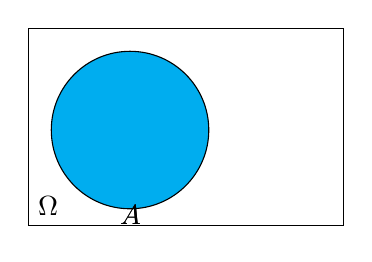
\begin{tikzpicture}[scale=0.5]
\draw  (-4,-1) rectangle (4,4);\node[above right] at (-4,-1) {$\Omega$};
\fill[color=cyan]  (0,0) ++(135:2) circle (2);\node at (-1.4,-0.75) {$A$};
\draw  (0,0) ++(135:2) circle (2);\node at (-1.4,-0.75) {$A$};
\end{tikzpicture}		\\
\hline
$\omega\in A$&	 $\omega$ appartient à $A$&	 Le résultat $\omega$ est une des réalisations possibles de $A$	&	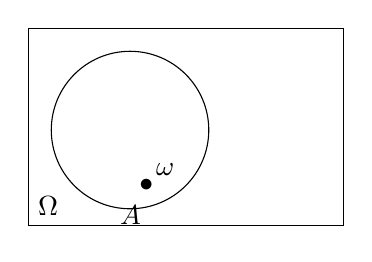
\begin{tikzpicture}[scale=0.5]
\draw  (-4,-1) rectangle (4,4);\node[above right] at (-4,-1) {$\Omega$};
\draw  (0,0) ++(135:2) circle (2);\node at (-1.4,-0.75) {$A$};
\node[above right] at (-1,0) {$\omega$};\node at (-1,0) {$\bullet$};
\end{tikzpicture}\\
\hline
 $A\subset B$&	 $A$ est inclus dans $B$&	 $A$ implique $B$&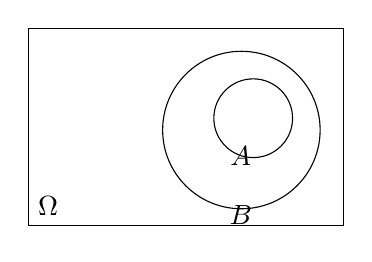
\begin{tikzpicture}[scale=0.5]
\draw  (-4,-1) rectangle (4,4);\node[above right] at (-4,-1) {$\Omega$};
\draw (0.3,0.3) ++(45:2) circle (1);\node at (1.4,0.75) {$A$};
\draw  (0,0) ++(45:2) circle (2);\node at (1.4,-0.75) {$B$};
\end{tikzpicture}	\\
\hline
 $A\cup B$&	réunion de $A$ et $B$&	 $A$ ou $B$	& 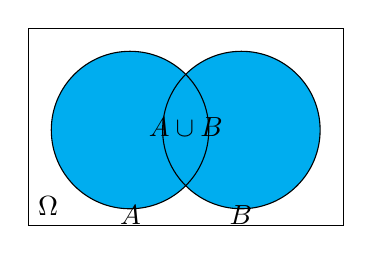
\begin{tikzpicture}[scale=0.5]
\draw  (-4,-1) rectangle (4,4);\node[above right] at (-4,-1) {$\Omega$};
\fill[color=cyan]  (0,0) arc(-135:135:2) arc(45:315:2);\node at (0,1.5) {$A\cup B$};
\draw  (0,0) ++(135:2) circle (2);\node at (-1.4,-0.75) {$A$};
\draw  (0,0) ++(45:2) circle (2);\node at (1.4,-0.75) {$B$};
\end{tikzpicture}\\
\hline
 $A\cap B$&	intersection de $A$ et $B$&	 $A$ et $B$&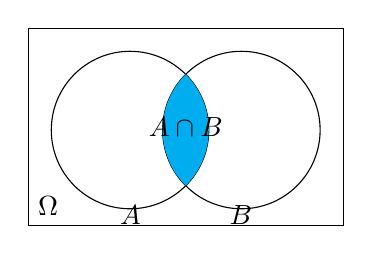
\begin{tikzpicture}[scale=0.5]
\draw  (-4,-1) rectangle (4,4);\node[above right] at (-4,-1) {$\Omega$};
\draw  (0,0) ++(135:2) circle (2);\node at (-1.4,-0.75) {$A$};
\draw  (0,0) ++(45:2) circle (2);\node at (1.4,-0.75) {$B$};
\fill[color=cyan]  (0,0) arc (-45:45:2) arc (135:225:2);\node at (0,1.5) {$A\cap B$};;
\end{tikzpicture}
 	\\
\hline
 $\bar A$ (noté aussi $A^{c}$)&	complémentaire de $A$ dans  $\Omega$	&	événement contraire de $A$&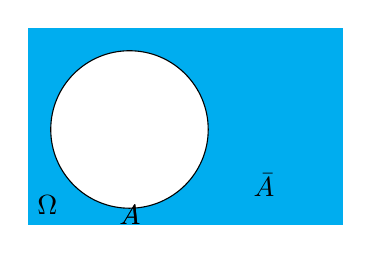
\begin{tikzpicture}[scale=0.5]
\fill[color=cyan]  (-4,-1) rectangle (4,4);\node[above right] at (-4,-1) {$\Omega$};
\fill[color=white]  (0,0) ++(135:2) circle (2);\node at (-1.4,-0.75) {$A$};
\draw  (0,0) ++(135:2) circle (2);\node at (-1.4,-0.75) {$A$};
\node at (2,0) {$\bar A$};
\end{tikzpicture}	\\
\hline
 $ A\cap B=\emptyset$&	 $A$ et $B$ sont disjoints&	$A$ et $B$ sont incompatibles&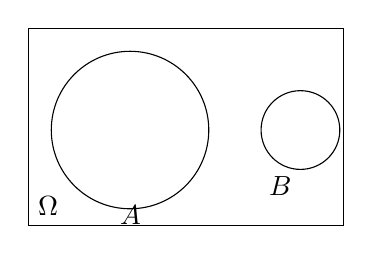
\begin{tikzpicture}[scale=0.5]
\draw  (-4,-1) rectangle (4,4);\node[above right] at (-4,-1) {$\Omega$};
\draw  (0,0) ++(135:2) circle (2);\node at (-1.4,-0.75) {$A$};
\draw (1.5,0) ++(45:2) circle (1);\node at (2.4,0) {$B$};
\end{tikzpicture}	\\
\hline
\end{tabular}
\end{center}
\end{Definition} 

\begin{Definition}[Tribu]
L'ensemble des événements possibles appelé \defi{tribu} est l'ensemble des parties de l'univers. Dans le cadre d'un univers fini, la tribu est l'ensemble des parties de l'univers, soit $\mathcal{P}(\Omega)$.
\end{Definition}
\begin{Exemple}
Pour le lancer d'une pièce, l'univers est $\{P,F\}$ et la tribu est $ \{\varnothing, \{P \}, \{F \}, \{P, F \} \}$.
\end{Exemple}

\begin{Definition}[Espace probabilisable]
Le couple $(\Omega,\mathcal{P}(\Omega))$ est appelé \defi{espace probabilisable}.
\end{Definition}

\begin{Definition}[Axiomes des probabilités]
Soit $(\Omega,\mathcal{P}(\Omega))$ un espace probabilisable fini.\\
Une \defi{probabilité}, $P$, sur $(\Omega,\mathcal{P}(\Omega))$ est une application :
\[ \Fonction{P}{\mathcal{P}(\Omega)}{\R^+}{A}{P(A)} \]
vérifiant :
\begin{itemize}
\item
  $P(\Omega)=1$.
\item
  Pour deux événements disjoints $A$ et $B$, on a  :
$$P(A\cup B)=P(A)+P(B).$$  
\end{itemize}
Le triplet  $(\Omega,\mathcal{P}(\Omega),P)$ s'appelle un \defi{espace probabilisé}.
\end{Definition}



\begin{Proposition}
\begin{enumerate}
\item $ P(\emptyset)=0.$
\item Pour tout $A,B\in \mathcal{P}(\Omega)$ tel que  $A\subset B$, on a :
$$P(A)\leq P(B)$$
$$P(B\setminus A )=P(B)-P(A)$$
\item Pour tout $A\in \mathcal{P}(\Omega)$, on a $P(A)\in[0,1]$.
\item Pour tout $A,B\in \mathcal{P}(\Omega)$, on a $$P(A\cup B)+P(A\cap B)=P(A)+P(B).$$
\item Pour tout $A,B\in \mathcal{P}(\Omega)$, on a $$P(A\cap B)\leq P(A)+P(B).$$
\item Si $A_1, \dots, A_n$ est une famille d'événements deux à deux incompatibles, alors
alors \[ P\left( \cup_{i=1}^n A_i \right) = \sum_{i=1}^n P(A_i) \]
\item Sous additivité : si $A_1, \dots, A_n$ est une famille d'événements , alors  :
\[ P\left( \cup_{i=1}^n A_i \right) \leq  \sum_{i=1}^n P(A_i) \]
\end{enumerate}
\end{Proposition}
\begin{Demonstration}
\begin{enumerate}
\item Les deux événements  $\Omega$ et $\emptyset$ sont disjoints d'où :
$$\begin{aligned}
P(\Omega)=&P(\Omega\cup \emptyset )\\
P(\Omega)=&P(\Omega)+P(\emptyset)\\
P(\emptyset)=&0.
\end{aligned}$$
\item Comme $A\subset B$, on a  $A \bigcup\limits_{\text{disjoints}}(B\setminus A)=B$, d'où :
$$ P(A)+P(B\setminus A)=P(B)$$
et 
$$ P(A)\leq P(B)$$
\item Comme $A\subset \Omega$, on a $P(A)\leq P(\Omega)=1$.
\item Comme $A\cup B=(A\setminus (A\cap B))\bigcup\limits_{\text{disjoints}}B$, on a $$P(A\cup B)=P(A\setminus (A\cap B))+P(B).$$ Comme $(A\cap B)\subset A$, on a bien : 
 $$P(A\cup B)=P(A)- P(A\cap B)+P(B).$$
\item Comme $P(A\cup B)+ P(A\cap B)=P(A)+P(B)$, on a $P(A\cup B)\leq P(A)+P(B)$.
\item Démonstration par récurrence :\\
Soit $H_n$ la propriété si $A_1, \dots, A_n$ est une famille d'événements deux à deux incompatibles,
alors \[ P\left( \cup_{i=1}^n A_i \right) = \sum_{i=1}^n P(A_i) \].
\begin{itemize}
\item $H_1$ : on a bien  $P(A)=P(A)$.
\item $H_n\Rightarrow H_{n+1}$ : Soit $A_1, \dots, A_n, A_{n+1}$ une famille d'événements deux à deux incompatibles. On a:
$$\begin{aligned}
P\left( \cup_{i=1}^{n+1} A_i \right)&=P(\left( \cup_{i=1}^{n} A_i \right)\cup A_{n+1} )\\
&=P\left( \cup_{i=1}^{n} A_i \right)+ P (A_{n+1} ) \text{ car } \cup_{i=1}^{n} A_i \text{ et } A_{n+1} \text{ sont disjoints} \\
&= \sum_{i=1}^n P(A_i)+ P (A_{n+1} ) \text{ car } H_n \\
&= \sum_{i=1}^{n+1} P(A_i).
\end{aligned}$$
\end{itemize}
\item Démonstration identique à la précédente en remplaçant les égalités par inégalités.
\end{enumerate}
\end{Demonstration}

\begin{DefinitionProposition}[Probabilité uniforme]
On appelle \defi{probabilité uniforme} sur $\Omega$ la probabilité définie par :
$$P(A)=\frac{\operatorname{Card} (A)}{\operatorname{Card} (\Omega)}.$$
\end{DefinitionProposition}
\begin{Demonstration}
\begin{itemize}
\item $P(\Omega)=\frac{\operatorname{Card} (\Omega)}{\operatorname{Card} (\Omega)}=1.$
\item Soit $A$ et $B$ deux parties disjointes de $\Omega$. On a :
$$P(A\cup B)=\frac{\operatorname{Card} (A\cup B)}{\operatorname{Card} (\Omega)}\overbrace{=}^{\text{A  et B sont disjoints}}=\frac{\operatorname{Card} (A)+ \operatorname{Card} (B)}{\operatorname{Card} (\Omega)}=\frac{\operatorname{Card} (A)}{\operatorname{Card} (\Omega)}+\frac{\operatorname{Card} (B)}{\operatorname{Card} (\Omega)}=P(A)+P(B) .$$

\end{itemize}
\end{Demonstration}
\begin{Exemple}[Lancer de deux dés]
Pour l'expérience aléatoire du lancer de deux dés, l'univers est $\Omega=\overbrace{\{1,2,3,4,5,6\}}^{\text{issues du premier dé}}\times \overbrace{\{1,2,3,4,5,6\}}^{\text{issues du second dé}}$ et la probabilité est la probabilité uniforme.\\
L'événement $A$="Somme des chiffres égale à 2 ou 12" est $\{(1,1),(6,6)\}$.\\
L'événement $B$="Somme des chiffres égale à 7" est $\{(1,6),(2,5),(3,4),(4,3),(5,2),(6,1)\}$. \\
D'où
$$P(A)=\frac{\operatorname{Card} (A)}{\operatorname{Card} (\Omega)}=\frac{2}{36}=\frac{1}{18},$$
et
 $$P(B)=\frac{\operatorname{Card} (B)}{\operatorname{Card} (\Omega)}=\frac{6}{36}=\frac{1}{6}.$$
\end{Exemple}

\begin{Proposition}[Détermination d'une probabilité par l'image des singletons]
Une probabilité $P$ sur un univers fini est complètement déterminée par les $P(\{\omega\})$ pour tout $\omega \in \Omega$.\\
$P(\{\omega\})$ est appelé \defi{poids de probabilité}.
\end{Proposition}
\begin{Demonstration}
En effet, pour $A \subset \Omega$, on a :
$$\begin{aligned}
P(A)&=P(\bigcup\limits_{\omega\in A}\{w\} ),\\
 &=\sum_{\omega\in A}P(\{w\}).
\end{aligned}$$
\end{Demonstration}
\begin{Remarque}
\begin{itemize}
\item Les poids d'une probabilité $P$ vérifient
$$ \sum_{\omega \in \Omega}P(\{\omega\}) = 1.$$
\item Il est souvent plus facile de définir une probabilité sur les événements élémentaires ("les issues") que sur l'ensemble des événements.
\item Une probabilité sur $\Omega=\Intf{1}{n}$ est la donnée d'une suite finie $(p_1,\ldots,p_n)$ de nombres tels que :
\begin{enumerate}
\item $p_i = P(\{\omega_i\}),\forall i\in\Intf{1}{n} $
\item $0\leq p_i\leq 1,,\forall i\in\Intf{1}{n}$
\item $p_1+p_2+\ldots+p_n=1.$
\end{enumerate}
\end{itemize}
\end{Remarque}
\begin{Exemple}
Une dé est pipé tel que la chance d'obtenir le chiffre 6 soit 2 fois plus grande que les autres chiffre. Dans ce cas, on a donc :
$$\begin{cases}
p_6=2 p_1=2 p_2=2 p_3=2 p_4=2 p_5 \\
p_1+p_2+p_3+p_4+p_5+p_6=1
\end{cases}$$
Après résolution de ce système d'équations, la probabilité est donc définie par
$$p_1=p_2=p_3=p_4=p_5=\frac 1 7 \text{ et }  p_6=\frac 2 7.$$
\end{Exemple}
Un système complet d'événements intervient dans la modélisation d'une expérience aléatoire à plusieurs étapes.
\begin{Definition}[Système complet d'événements]
Soit $(\Omega,\mathcal{P}(\Omega),P)$ un espace probabilisé.\\
Un \defi{système complet d'événements}, appelé aussi \defi{partition}, est une famille $(A_1,\ldots,A_n)$
d'événements deux à deux incompatibles tels que
\[ \bigcup\limits_{i=1}^n A_i = \Omega . \]
\begin{center}
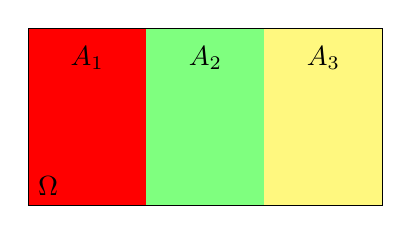
\begin{tikzpicture}[scale=0.75]

%\fill[color=cyan!50] (0,1.5) ellipse (2.5 and 2);
\fill[red] (-3,-1) rectangle (-1,2);\node at (-2,1.5) {$A_1$};
\fill[opacity=0.5,green] (-1,-1) rectangle (1,2);\node at (0,1.5) {$A_2$};
\fill[opacity=0.5,yellow] (1,-1) rectangle (3,2);\node at (2,1.5) {$A_3$};
\draw (-3,-1) rectangle (3,2);\node[above right] at (-3,-1) {$\Omega$};
\end{tikzpicture}\\
$(A_1,A_2,A_3)$ est un système complet d'événements de $\Omega$.
\end{center}
\end{Definition}
\begin{Remarque}[$A,\bar A$ système complet d'événements]
$(A,\bar A)$ est un système complet d'événements pour tout événement $A$.
\end{Remarque}


\begin{Proposition}[Probabilité d'un système complet d'événements]
\label{prop:sce}
Soit $(\Omega,\mathcal{P}(\Omega),P)$ un espace probabilisé.\\
Soit $(A_1,\ldots,A_n)$ un système complet d'événements.\\
On a :
\[ 1 = \sum_{i=1}^n P(A_i). \]
Pour tout événement $B$, on a
\[ P(B) = \sum_{i=1}^n P(B\cap A_i). \]
\begin{center}
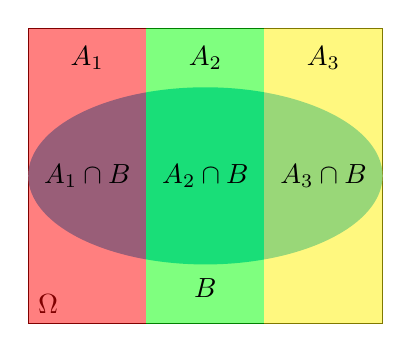
\begin{tikzpicture}[scale=0.75]
\draw (-3,-1) rectangle (3,4);\node[above right] at (-3,-1) {$\Omega$};
\fill[color=cyan!80] (0,1.5) ellipse (3 and 1.5);
\fill[opacity=0.5,red] (-3,-1) rectangle (-1,4);\node at (-2,3.5) {$A_1$};
\fill[opacity=0.5,green] (-1,-1) rectangle (1,4);\node at (0,3.5) {$A_2$};
\fill[opacity=0.5,yellow] (1,-1) rectangle (3,4);\node at (2,3.5) {$A_3$};
\node at (0,1.5) {$A_2\cap B$};
\node at (-2,1.5) {$A_1\cap B$};
\node at (2,1.5) {$A_3\cap B$};
\node at (0,-0.4) {$B$};
\end{tikzpicture}
\end{center}

\end{Proposition}




\begin{Demonstration}
On a :
$$\begin{aligned}
P(B)&=P(B\cap \Omega )\\
P(B)&=P(B\cap \left(\bigcup\limits_{i=1}^n A_i\right ) )\\
P(B)&=P(\bigcup\limits_{i=1}^n (B\cap A_i))\\
P(B)&=\sum_{i=1}^n P(B\cap A_i).
\end{aligned}$$
En particulier si $B=\Omega$, on a :
$$\begin{aligned}
P(\Omega)&=\sum_{i=1}^n P(\Omega\cap A_i)\\
1&=\sum_{i=1}^n P(A_i)
\end{aligned}$$
\end{Demonstration}
\begin{Remarque}
En particulier, pour tout événement $A$, on a :
$$P(A)+P(\bar A)=1$$
et pour tout événement $B$, :
$$P(B) = P(B\cap A)+P(B\cap\bar A)$$
\end{Remarque}
\begin{Exemple}[3 urnes]
On dispose de 3 urnes $U_1$, $U_2$, $U_3$, chacune contient 10 boules; parmi elles, $U_1$ contient 1 blanche, $U_2$ contient 2 blanches, et $U_3$ contient 6 blanches. On tire au hasard une urne puis  une boule dans cette urne. Quelle est la probabilité de l'événement $B$="obtenir une blanche" ?\\
Les événements $U_1$="tirer l'urne 1,  $U_2$="tirer l'urne 2", $U_3$="tirer l'urne 3" forment un système complet d'événements. On a donc :
$$P(B)= P(B\cap U_1)+P(B\cap U_2)+P(B\cap U_3).$$
Le but des probabilités conditionnelles est de déterminer les probabilités des termes de cette somme.
\end{Exemple}

\subsection{Probabilité conditionnelle}
Dans l'expérience aléatoire des trois urnes, la probabilité de tirer une boule blanche est modifiée si l'on dispose de l'information l'urne 1 a été choisie.  
Le concept de probabilité conditionnelle permet de prendre en compte ce complément d'information.\\
Par exemple, une classe est constituée de $N$ élèves, dont 
\begin{enumerate}
\item $N_h$ hommes,
\item $N_m$ majeurs,
\item $N_{h\cap m}$ hommes et majeurs.
\end{enumerate}
Un élève passant au tableau est choisi aléatoirement. \\
On note $H=$"élève choisi est un homme" et  $M=$"élève choisi est majeur".\\
L'équiprobabilité donne  :
$$ P(M) = \frac{N_m}{N}\text{ et } P(H\cap M)=\frac{N_{h\cap m}}{N}.$$
Quelle est la probabilité que l'élève choisie soit un homme sachant qu'il doit être majeur, noté $P_M(H)$ ? \\
Dans cette expérience aléatoire, l'information supplémentaire est l'élève choisi  est majeur. L'univers est maintenant l'ensemble des élèves majeurs donc la probabilité est :
$$P_M(H) =\frac{N_{h\cap m}}{N_m}.$$
Mais,
$$P_M(H) =\frac{N_{h\cap m}}{N_m}=\frac{\frac{N_{h\cap m}}{N}}{\frac{N_m}{N}}=\frac{P(H\cap M)}{P(M)}.$$ 
Par analogie, la définition formelle est :
\begin{Definition}[Probabilité conditionnelle]
Soit $(\Omega,\mathcal{P}(\Omega),P)$ un espace probabilisé.
Soit $A$ un événement tel que $P(A)>0$.\\
L'application
\[ \Fonction{P_A}{\mathcal{P}(\Omega)}{[0,1]}{B}{\frac{P(A\cap B)}{P(A)}} \]
est une probabilité sur $(\Omega,\mathcal{P}(\Omega))$
appelée \defi{probabilité conditionnellement à $A$},
ou \defi{probabilité sachant $A$}.\\
On note $P(B|A) = P_A(B)$.
\end{Definition}

\begin{Exemple}
On lance un dé parfaitement équilibré. La probabilité d'obtenir un 6 est 1/6. On suppose maintenant que ce dé a ses faces impaires peintes en vert, et ses faces paires peintes en bleu. On a aperçu de loin que, sur le dessus du dé, on a obtenu une face bleue. Quelle est la probabilité d'obtenir 6 sachant une face bleue ?\\
On note $B=\{2,4,6\}$ l'événement "face bleue". On a :
$$P_B(\{6\})=\frac{P(\{6\}\cap B)}{P(B)}=\frac{\frac{\operatorname{Card}( \{6\})}{\operatorname{Card}( \Omega)} }{\frac{\operatorname{Card}( \{2,4,6\})}{\operatorname{Card}( \Omega)} }=\frac{\frac 1 6 }{\frac 3 6 }=\frac 1 3.$$
\end{Exemple}


\begin{Proposition}[Formule des probabilités totales]
Soit $(\Omega,\mathcal{P}(\Omega),P)$ un espace probabilisé.\\
Soit $(A_1,\ldots,A_n)$ un système complet d'événements de probabilités non nulles.\\
Pour tout événement $B$, on a
\[ P(B) = \sum_{i=1}^n P_{A_i}(B)P(A_i). \]
\end{Proposition}
\begin{Demonstration}
Dans l'équation d'un système complet d'événements  de la proposition~\ref{prop:sce}, il suffit de remplacer $P(B\cap A_i)$ pat $P(B|A_i)P(A_i).$
\end{Demonstration}
\begin{Exemple}[3 urnes]
La probabilité de tirer une boule blanche était de :
$$P(B)= P(B\cap U_1)+P(B\cap U_2)+P(B\cap U_3).$$
Ce qui donne :
$$P(B)= P_{U_1}(B)P(U_1)+P_{U_1}(B)P(U_2)+P_{U_3}(B)P(U_3)=\frac{1}{10} \frac 1 3+ \frac{2}{10} \frac 1 3 +\frac{3}{10} \frac 1 3 =\frac{6}{30} =\frac{1}{5} .$$
\end{Exemple}
\begin{Remarque}
En particulier, si  $A$ et $\bar A$ sont deux événements de probabilité non nulle, on a pour tout événement $B$:
\[ P(B) = P_A(B)P(A) + P_{\bar A}(B)P(\bar A).\]
\end{Remarque}



\begin{Proposition}[Formule de Bayes]
Soit $(\Omega,\mathcal{P}(\Omega),P)$ un espace probabilisé.\\
Soit $A$ et $B$ deux événements de probabilités non nulles.\\
Alors
$$ P_B(A) = \frac{ P_A(B)P(A) }{ P(B) }.$$
Cette formule permet d'inverser des conditions. 
\end{Proposition}
\begin{Demonstration}
On a $P(A\cap B)=P(B)P_B(A)$ et $P(A\cap B)=P(B\cap A)=P(A)P_A(B)$. Comme $P(B)\neq 0$, on a le résultat voulu. 
\end{Demonstration}

\begin{Proposition}[Formule de Bayes usuelle]
Soit $(\Omega,\mathcal{P}(\Omega),P)$ un espace probabilisé.\\
Soit $(A_1,\ldots,A_n)$ un système complet d'événements de probabilités non nulles.\\
Pour tout événement $B$ de probabilité non nulle,
et  on a
\[\forall k\in\Intf{1}{n} :\quad P_B(A_k) = \frac{ P_{A_k}(B)P(A_k) }{ \sum_{i=1}^n P_{A_i}(B)P(A_i) }. \]
\end{Proposition}

\begin{Remarque}
Le système $(A_1,\ldots,A_n)$ représente souvent une liste de causes pouvant amener l'événement B lors d'une étape
suivante de l'expérience par exemple dans le problème des 3 urnes. Il est alors généralement facile de déterminer la probabilité qu'une certaine
conséquence $B$ ait lieu, sachant que la cause $A_i$ a eu lieu, c'est-à-dire la probabilité conditionnelle
$P_{A_i}(B)$ en respectant l'ordre temporel. Ces données permettent, grâce à la formule de
Bayes, de remonter le temps, en déterminant la probabilité qu'une certaine cause $A_i$ ait eu lieu sachant
la conséquence $B$. Pour cette raison, cette formule est aussi souvent appelée formule de probabilité des
causes.
\end{Remarque}
\begin{Exemple}[3 urnes]
On cherche à connaître la probabilité que l'urne 1 est été choisie sachant que l'on a tiré une boule blanche, c'est à dire $P_B(U_1)$.\\
On a donc 
$$ P_B(U_1) = \frac{ P_{U_1}(B)P(U_1) }{  P_{U_1}(B)P(U_1)+ P_{U_2}(B)P(U_2)+ P_{U_3}(B)P(U_3) }=\frac{\frac{1}{3}\frac{1}{10}}{\frac{1}{3}\frac{1}{10}+\frac{1}{3}\frac{2}{10}+\frac{1}{3}\frac{6}{10}}=\frac{1}{9}.$$
\end{Exemple}


\begin{Exemple}[Test de dépistage]
Vous êtes directeur de cabinet du ministre de la santé. Une maladie est présente dans la population, dans la proportion d'une personne malade sur 10000. Un responsable d'un grand laboratoire pharmaceutique vient vous vanter son nouveau test de dépistage : si une personne est malade, le test est positif à 99$\%$. Si une personne n'est pas malade, le test est positif à 0,1$\%$.
  Ces chiffres ont l'air excellent, vous ne pouvez qu'en convenir. Toutefois, avant d'autoriser la commercialisation de ce test, vous faites appel au statisticien du ministère : ce qui vous intéresse, ce n'est pas vraiment les résultats présentés par le laboratoire, c'est la probabilité qu'une personne soit malade si le test est positif. La formule de Bayes permet de calculer cette probabilité.\\
  On note M l'événement : "La personne est malade", et T l'événement : "Le test est positif". Le but est de calculer $P_T(M)$. Les données que vous avez en main sont $P(M)=0,0001$ (et donc $P(\bar M)=0,9999$), $P_M(T)=0,99$ et $P_{\bar M}(T)=0,001$. La formule de Bayes donne :
$$P_T( \bar M)=\frac{P_{\bar M}(T)P(\bar M)}{P_M(T)P(M)+P_{\bar M}(T)P(\bar M)}=\frac{0,9999×10^{-3}}{10^{-4}0,99+0,9999×10^{-3}}\approx 0,91.$$
C'est catastrophique! Il y a que 91$\%$ de chances qu'une personne positive au test ne soit pas malade! C'est tout le problème des tests de dépistage pour des maladies rares : ils doivent être excessivement performants, sous peine de donner beaucoup trop de "faux-positifs".
\end{Exemple}


\begin{Definition}[Arbre de probabilité]
Un \defi{arbre de probabilité} est un schéma permettant de résumer une expérience aléatoire connaissant des probabilités conditionnelles, soit un graphe orienté et pondéré obéissant aux règles suivantes :
\begin{enumerate}
\item la somme des probabilités des branches issues d'un même sommet donne 1,
\item la probabilité d'un chemin est le produit des probabilités des branches qui le composent,
\item la probabilités de la branche allant du sommet A vers le sommet B est la probabilité conditionnelle de $B$ sachant que $A$ est déjà réalisé $P_A(B)$.
\end{enumerate}
On retrouve alors la propriété de la probabilité conditionnelle :
$$ P(A\cap B)= P_{A}(B)P(A).$$
Ainsi que la formule des probabilités totales, si $A_1, A_2, \dots , A_n$ définit un système complet d'évènements de probabilité non nulles, on a :
$$ P(B)=\sum _{i=1}^{n}P(B\cap A_{i})=\sum _{i=1}^{n} P_{A_{i}}(B)P(A_{i}).$$
\end{Definition}
%
\begin{Exemple}[3 urnes]
\begin{center}
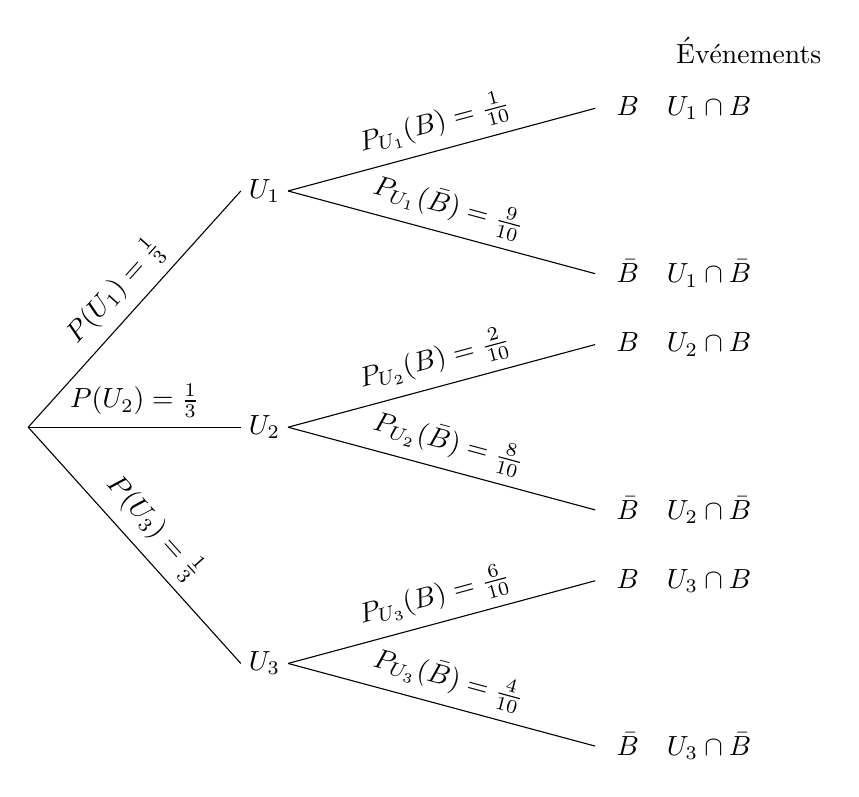
\begin{tikzpicture}[scale=1.5]
\draw (6.1,3) node[above]{\'Evénements};
\draw  (0,0)  -- (1.8,2) node[midway,sloped,above]{$P(U_1)=\frac 1 3 $};
\draw (2,2) node {$U_1$} ;
\draw  (2.2,2) -- (4.8,1.3)node[midway,sloped,above]{$P_{U_1}(\bar{B})=\frac{9}{10}$};
\draw (4.9,1.3) node[right] {$\bar{B}\quad U_1\cap \bar{B}$} ;    
\draw  (2.2,2) -- (4.8,2.7)node[midway,sloped,above]{$P_{U_1}(B)=\frac{1}{10}$};
\draw (4.9,2.7) node[right] {$B\quad U_1\cap B$} ;

\draw  (0,0) -- (1.8,0)node[midway,sloped,above]{$P(U_2)=\frac 1 3 $};
\draw (2,0) node {$U_2$} ;
\draw  (2.2,0) -- (4.8,-0.7)node[midway,sloped,above]{$P_{U_2}(\bar{B})=\frac{8}{10}$};
\draw (4.9,-0.7) node[right] {$\bar{B}\quad U_2\cap \bar{B}$} ;    
\draw  (2.2,0) -- (4.8,0.7)node[midway,sloped,above]{$P_{U_2}(B)=\frac{2}{10}$};
\draw (4.9,0.7) node[right] {$B\quad U_2\cap B$} ;

\draw  (0,0) -- (1.8,-2)node[midway,sloped,above]{$P(U_3)=\frac 1 3 $};
\draw (2,-2) node {$U_3$} ;
\draw  (2.2,-2) -- (4.8,-2.7)node[midway,sloped,above]{$P_{U_3}(\bar{B})=\frac{4}{10}$};
\draw (4.9,-2.7) node[right] {$\bar{B}\quad U_3\cap \bar{B}$} ;    
\draw  (2.2,-2) -- (4.8,-1.3)node[midway,sloped,above]{$P_{U_3}(B)=\frac{6}{10}$};
\draw (4.9,-1.3) node[right] {$B\quad  U_3\cap B$} ;
\end{tikzpicture}
\end{center}
La probabilité de  l'événement $B$ est la somme des probabilités des parcours
qui mènent à B, d'où 
$$P(B)= P_{U_1}(B)P(U_1)+P_{U_1}(B)P(U_2)+P_{U_1}(B)P(U_3).$$
\end{Exemple}
\begin{Proposition}[Formule des probabilités composées]
Soit $A_1,A_2,\dots, A_n$ $n$ événements vérifiant $P(A_1\cap A_2\cap \dots \cap A_{n-1})\neq 0$.\\
Alors 
$$P(A_1\cap A_2\cap \dots \cap A_{n})=P(A_1)P_{A_1}(A_2)P_{A_1\cap A_2 }(A_3)\dots P_{A_1\cap A_2\cap \dots \cap A_{n-1}}(A_n).$$
\begin{center}
\begin{tikzpicture}[scale=1.5]
\node (start) at (0,0) {$\Omega$};
\node (A1) at (1.5,1) {$A_1$};
\node (A1f) at (1.5,0) {};
\node (A2) at (3,2) {$A_2$};
\node (A2f) at (3,1) {};
\node (A3) at (4.5,3) {};
\node (A3f) at (4.5,2) {};
\node (A4) at (7.2,3) {$A_3:\quad P(A_1\cap A_2\cap A_{3})=P(A_1)P_{A_1}(A_2)P_{A_1\cap A_2 }(A_3)$};
\draw(start) -- (A1)node[midway,sloped,above]{$P(A_1)$};
\draw[dashed] (start) -- (A1f);
\draw(A1) -- (A2)node[midway,sloped,above]{$P_{A_1}(A_2)$};
\draw[dashed] (A1) -- (A2f);
\draw(A2) -- (A3)node[midway,sloped,above]{$P_{A_1\cap A_2}(A_3)$};
\draw[dashed] (A2) -- (A3f);
\end{tikzpicture}
Cas pour n=3
\end{center}
\end{Proposition}
\begin{Demonstration}
Démontrons par récurrence la propriété $(H_n)$ pour tout $n\in\N^*$ :
\begin{center}
Si $A_1,A_2,\dots, A_n$ $n$ événements vérifiant $P(A_1\cap A_2\cap \dots \cap A_{n-1})\neq 0$,\\
Alors  $P(A_1\cap A_2\cap \dots \cap A_{n})=P(A_1)P_{A_1}(A_2)P_{A_1\cap A_2 }(A_3)\dots P_{A_1\cap A_2\cap \dots \cap A_{n-1}}(A_n).$
\end{center}
\begin{itemize}
\item \textit{Initialisation : } Soit $A_1$ un événement. On a bien $P(A_1)=P(A_1)$.
\item \textit{Hérédité : } Soit $n\in\N^*$. Supposons la propriété $(H_n)$ vraie au rang $n$ et vérifions au rang $n+1$.\\
Soit $A_1,A_2,\dots, A_{n+1}$ $n+1$ événements vérifiant $P(A_1\cap A_2\cap \dots \cap A_{n})\neq 0$. \\
Comme  $P(A_1\cap A_2\cap \dots \cap A_{n})\neq 0$, on a :
$$P(A_1\cap A_2\cap \dots \cap A_{n} \cap A_{n+1})=P(A_1\cap A_2\cap \dots \cap A_{n}) P_{A_1\cap A_2\cap \dots \cap A_{n}}(A_n+1).$$
Comme  $A_1\cap A_2\cap \dots \cap A_{n} \subset A_1\cap A_2\cap \dots \cap A_{n-1}$, on a $P(A_1\cap A_2\cap \dots \cap A_{n-1})\neq 0$. On applique l'hypothèse de récurrence à $P(A_1\cap A_2\cap \dots \cap A_{n})$, d'où 
$$P(A_1\cap A_2\cap \dots \cap A_{n} \cap A_{n+1})=P(A_1)P_{A_1}(A_2)P_{A_1\cap A_2 }(A_3)\dots P_{A_1\cap A_2\cap \dots \cap A_{n-1}}(A_n) P_{A_1\cap A_2\cap \dots \cap A_{n}}(A_n+1).$$
\end{itemize}
La propriété $(H_n)$ est donc vraie pour tout $n\in\N^*$.
\end{Demonstration}
\begin{Exemple}
On considère une urne contenant 4 boules blanches et 3 boules noires. On tire une à une et sans remise 3 boules de l'urne. Quelle est la probabilité pour que la première boule tirée soit blanche, la seconde blanche et la troisième noire ?\\
On note $B_i$  l'événement : "La i-ème boule tirée est blanche (resp. noire)". On cherche à calculer $P(B_1\cap B_2 \cap \bar B_3)$, ce que l'on va faire en utilisant la formule des probabilités composées :
$$P(B_1\cap B_2 \cap \bar B_3)=P(B_1)P(B_2|B_1)P(\bar B_3|B_1\cap B_2).$$
Chacune des probabilités qui apparaît est facile à calculer, car $P(B_1)=4/7$, $P(B_2|B_1)=3/6$ (il reste 6 boules dont 3 blanches) et $P(\bar B_3|B_1\cap B_2)=3/5$. Finalement, on obtient $P(B_1\cap B_2 \cap \bar B_3)=6/35$.
\end{Exemple}
% -----------------------------------------------------------------------------
\subsection{Indépendance}
On considère l'expérience aléatoire de lancer successivement deux fois un dé.\\
Soit  $A$ un événement relié au premier lancer, par exemple obtenir un chiffre pair sur le premier dé et 
soit  $B$ un événement relié au second lancer, par exemple obtenir un chiffre impair sur le second dé.
L'information de savoir que l'événement $A$ est réalisé, ne modifie pas la probabilité de l'événement $B$, autrement dit $P_A(B) = P(B)$. 
Mais, d'après la définition de la probabilité conditionnelle, on a : $P_A(B) =\frac{P(A\cap B)}{P(A)}$. De ces deux égalités, on obtient $P(A\cap B)=P(A)P(B)$ et on dit que les deux événements sont indépendants.\\ 
Par analogie, la définition formelle est :
\begin{Definition}[Indépendance]

Soit $(\Omega,\mathcal{P}(\Omega),P)$ un espace probabilisé.
\begin{itemize}
\item
  Deux événements $A$ et $B$ sont \defi{indépendants} si $P(A\cap B)=P(A)P(B)$.
\item
  Une famille $(A_1,\ldots,A_n)$ d'événements sont \defi{(mutuellement) indépendants}
  si pour toute partie $I\subset\Intf{1}{n}$, on a
  \[ P\left( \bigcap_{i\in I} A_i \right) = \prod_{i\in I} P(A_i).\]
\end{itemize}
\end{Definition}
\begin{Exemple}[Lancer de deux dés]
$A$="Obtenir 5 ou 6 sur le premier dé"\\
$A=\{(5,1),(5,2),(5,3),(5,4),(5,5),(5,6),(6,1),(6,2),(6,3),(6,4),(6,5),(6,6)\}$.\\
$B$="Obtenir  6 sur le second dé"\\
$B=\{(1,6),(2,6),(3,6),(4,6),(5,6),(6,6)\}$\\
$A\cap B=$"Obtenir 5 ou 6 sur le premier dé et obtenir  6 sur le second dé".\\
$A\cap B= \{ (5,6),(5,6),(6,6)\}.$
On a $P(A)=\frac{12}{36}=\frac 1 3 , P(B)=\frac{6}{36}=\frac 1 6$ et $P(A\cap B)=\frac{3}{36}=\frac{1}{12}= P(A)P(B)$.\\
Donc les événements $A$ et $B$ sont indépendants.
\end{Exemple}

\begin{Remarque}
Trois événements peuvent être indépendants deux à deux, sans pour autant être mutuellement indépendants. 
Par exemple, on considère un dé équilibré à 4 faces. On a $\Omega=\{1,2,3,4\}$ avec $p_1=p_2=p_3=p_4=\frac 1 4$.\\
Soit les événements $A=\{1,2\}, B=\{1,3\}$ et $C=\{1,4\}.$\\
On a : $$P(A)=P(B)=P(C)=\frac 1 2$$ et $$P(A\cap B)=P(A\cap C)=P(B\cap C)=P(\{1\})=\frac 1 4 =P(A)P(B)=P(A)P(C)=P(B)P(C).$$
Les événements $A$, $B$ et $C$ sont deux à deux indépendants mais :
 $$P(A\cap B\cap C )= P(\{1\})=\frac 1 4 \neq  \frac 1 8 =  P(A)P(B)P(C).$$
 Donc les événements ne sont pas mutuellement indépendants.
\end{Remarque}
\begin{Proposition}[Lien avec la probabilité conditionnelle]
Soit $(\Omega,\mathcal{P}(\Omega),P)$ un espace probabilisé.\\
Soit $A$ un événement de probabilité non nulle
et $B$ un événement quelconque.\\
Alors les événements $A$ et $B$ sont indépendants si et seulement si $P_A(B)=P(B)$.
\end{Proposition}
\begin{Demonstration}
Soit $A$ et $B$ deux événements tel que $P(A)\geq 0$.\\
$$\begin{aligned}
A, B \text{ sont indépendants } & \Leftrightarrow P(B\cap A)=P(B)P(A)\\
& \Leftrightarrow \frac{P(B\cap A)}{P(A)}=P(B) \text{ car }P(A)\neq 0\\
& \Leftrightarrow P_A(B)=P(B).
\end{aligned}$$ 
\end{Demonstration}




%TODO voir cours de mpsi sur les méthodes



\section{Variable aléatoire}
\begin{Exemple}[Jeu]Pour attirer les clients, un casino propose un nouveau jeu : le croupier lance simultanément 2 dés et calcule leur somme,
\begin{itemize} 
\item si la somme est égale à 2 ou 12, le joueur gagne 2 euros,
\item si la somme est égale à 7, le casino gagne 1 euro,
\item dans les autres cas, c'est nul (le joueur gagne 0 euro).  
\end{itemize}
A votre avis, ce jeu est-il favorable au joueur ou au casino ? Quel est le gain moyen du joueur ?


Dans ce jeu, on fait intervenir le hasard en observant la somme des points marqués par deux dés. Considérons le jet d'un dé bleu et d'un dé
rouge et notons $S$ la somme des points obtenus. On modélise cette expérience
en prenant l'équiprobabilité sur l'univers  
$$\Omega=\overbrace{\{1,2,3,4,5,6\}}^{\text{issues du dé bleu}}\times \overbrace{\{1,2,3,4,5,6\}}^{\text{issues du dé rouge}}.$$
Une issue, $\omega$, est un couple $(b, r)$ où b désigne le chiffre du
dé bleu et r celui du rouge. La somme $S$ est l'application :
$$\Fonction{S}{\Omega}{\{2,3,\dots,12\} }{(b, r)}{b+r}$$ 
Cette application est représentée par ce tableau  : 
\begin{center}
\begin{tabular}{c||c|c|c|c|c|c}
 $b\textbackslash r$ & 1 & 2&3&4&5&6 \\\hline\hline
1 & 2 & 3 & 4&5&6&7\\
2 & 3 & 4 & 5&6&7&8\\
3 & 4 & 5 & 6&7&8&9\\
2 & 5 & 6 & 7&8&9&10\\
1 & 6 & 7 & 8&9&10&11\\
2 & 7 & 8 & 9&10&11&12\\
\end{tabular}
\end{center}
On dit que S est une variable aléatoire sur $\{2,3,\dots,12\}$.\\
En fait, l'observation qui nous intéresse dans cette expérience, ce n'est pas $\omega$,  mais seulement $S(\omega)$. On aimerait connaître la probabilité que
la somme des points prenne une valeur donnée, soit $P(S = k)$ pour $k$ entier
fixé entre 2 et 12. \\
La méthode est de déterminer l'ensemble des issues donnant $(S=k)$ en lisant le tableau ci-dessous puis de calculer la probabilité de cet événement. Par exemple, on a $(S=3)=\{(1,2),(2,1)\}$, puis $$P(S=3)=P(\{(1,2),(2,1)\})\overbrace{=}^{\text{équiprobabilité}}\frac{\operatorname{Card}(\{(1,2),(2,1)\}) }{\operatorname{Card}(\Omega)}=\frac{2}{36}.$$
On obtient ainsi :
\begin{center}
\begin{tabular}{|c||c|c|c|c|c|c|c|c|c|c|c|}
\hline
$k$ & 2 & 3& 4& 5& 6& 7& 8& 9& 10& 11& 12 \\\hline
$P(S=k)$ & $\frac{1}{36}$ & $\frac{2}{36}$& $\frac{3}{36}$& $\frac{4}{36}$& $\frac{5}{36}$& $\frac{6}{36}$& $\frac{5}{36}$& $\frac{4}{36}$& $\frac{3}{36}$& $\frac{2}{36}$& $\frac{1}{36}$\\\hline
\end{tabular}
\end{center}
Cela revient à considérer un nouvel univers :
$$\Omega'=\{2, 3, 4, 5, 6, 7, 8, 9, 10, 11, 12\}$$
et à munir cet ensemble de la probabilité $P_S$ définie par le tableau des $P(S =
k)$. Cette nouvelle probabilité s'appelle loi de la variable aléatoire S.
\end{Exemple}

\subsection{Définition}

\begin{Definition}[Variable aléatoire]
Soit $(\Omega,\mathcal{P}(\Omega),P)$ un espace probabilisé fini.\\
Une \defi{variable aléatoire réelle} est une application : $$\Fonction{X}{\Omega}{\R}{\omega}{X(\omega)}.$$
On note $X(\Omega)=\{X(\omega):\omega \in \Omega \}$ l'ensemble des images de la variable aléatoire.\\
Comme $\Omega$ est fini, $X(\Omega)$ est aussi finie. On s'autorise désormais à écrire l'ensemble des images sous la forme $X (\Omega) = \{x_1,x_2,\dots,x_n\}$.
\end{Definition}
\begin{Remarque}
\begin{itemize}
\item Malgré son nom, une variable aléatoire n'est pas une variable (c'est une fonction) et elle n'est pas aléatoire.
\item Il est toujours possible de quantifier les valeurs prises par une variable aléatoire. Par exemple si $X$ représente le sexe de l'enfant à la naissance, on posera le label 1 pour le sexe féminin et le label 0 pour le sexe masculin et dans ce cas $X(\Omega)=\{0,1\}$.
\item Dans ce cours l'espace de probabilité  est finie et la variable aléatoire  réelle, on écrira "Soit $X$ une variable aléatoire" au lieu de "Soit $X$ une variable aléatoire réelle sur un espace probabilisé fini $(\Omega,\mathcal{P}(\Omega),P)$."
\end{itemize}
\end{Remarque}
\begin{Exemple}[Variable aléatoire indicatrice de $A$]
Soit $A$ un événement de $\Omega$.\\
La variable aléatoire indicatrice de $A$, noté $1_A$,  est une fonction  explicitant l'appartenance ou non à un événement $A$ 
de toute issue de $\Omega$ :
$$\Fonction{1_A}{\Omega}{\{0,1\}}{\omega}{\begin{cases}1&\text{si }\omega\in A \\0&\text{si }\omega\notin A
\end{cases}}.$$
\end{Exemple}

\begin{Definition}[Événements associés à une variable aléatoire]
Soit $X$ une variable aléatoire.\\
Pour tout $A\subset \R$, on définit l'événement $\{ X \in A \}$ comme étant
\[ X^{-1}(A) = \{\omega\in\Omega :   X(\omega )\in A\}. \]
Dans le cadre de ce chapitre, nous aurons recours aux notations suivantes, pour $x \in \R$ et $A \subset \R$ :
$$\begin{aligned}
(X\in A)=&X^{-1}(A)=\{\omega  \in \Omega | X (\omega) \in A\}\\
(X = x ) =& X^{-1}(\{x\}) = \{\omega \in \Omega | X (\omega) = x \}\\
(X \leq x ) =& X^{-1}(]-\infty,x]) = \{\omega \in \Omega | X (\omega) \leq x \}\\
(X < x ) =& X^{-1}(]-\infty,x[) = \{\omega \in \Omega | X (\omega) < x \}\\
(X \geq x ) =& X^{-1}([x,+\infty[) = \{\omega \in \Omega | X (\omega) \geq x \}\\
(X > x ) =& X^{-1}(]x,+\infty[) = \{\omega \in \Omega | X (\omega) > x \}\\
\end{aligned}$$
\end{Definition}
\begin{Remarque}
Dans les démonstrations, sans perte de généralité, on considérera uniquement les parties de $X(\Omega)$ et non de $\R$ pour les rendre plus lisibles.
\end{Remarque}
\begin{Exemple}[Jeu]
Par exemple, l'ensemble des issues donnant une somme à 7 est :
$$\{S=7\}= S^{-1}(\{7\})=\{(1,6),(2,5),(3,4),(4,3),(5,2),(6,1)\}.$$
et l'ensemble des issues donnant une somme à 2 ou 12 est :
$$\{S\in \{2,12\}\}= S^{-1}(\{2,12\})=\{(1,1),(6,6)\}.$$
\end{Exemple}
\begin{Proposition}
Soit $X$ une variable aléatoire.\\
L'ensemble $(X=x_i)_{1\leq i\leq n}$ forme un système complet d'événements de $\Omega$.
\begin{center}
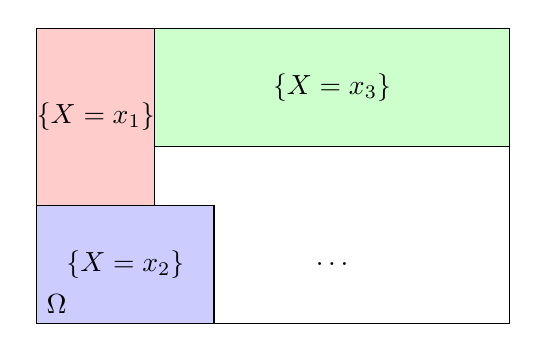
\begin{tikzpicture}[scale=0.75]
\draw[fill=red!20] (-4,1) rectangle (-2,4) node[pos=.5] {$\{X=x_1\}$} ;
\draw[fill=blue!20] (-4,-1) rectangle (-1,1)node[pos=.5] {$\{X=x_2\}$};
\draw[fill=green!20] (-2,2) rectangle (4,4) node[pos=.5] {$\{X=x_3\}$} ;
\draw (1,0) node  {$\dots$} ;
\draw (-4,-1) rectangle (4,4);\node[above right] at (-4,-1) {$\Omega$};
\end{tikzpicture} 
\end{center}
\end{Proposition}
\begin{Demonstration}
\begin{itemize}
\item \textit{disjoints :} Soit $i\neq j$. $\{i\}$ et $\{j\}$ sont deux ensembles disjoints. Donc $X^{-1}(\{i\})$ et $X^{-1}(\{j\})$ sont aussi disjoints.   
\item $\cup_{i=1}^n (X=x_i)=\cup_{i=1}^n X^{-1}(\{x_i\})\overbrace{=}^{\text{Formule de Hausdorff}} X^{-1}(\cup_{i=1}^n\{x_i\})=X^{-1}(X(\Omega))=\Omega.$ 
\end{itemize}
\end{Demonstration}

\subsection{Loi de probabilité}
\begin{DefinitionProposition}[Loi d'une variable aléatoire]
Soit $X$ une variable aléatoire.\\
L'application
\[ \Fonction{P_X}{\mathcal{P}(X(\Omega))}{\R^+}{A}{P(X^{-1}(A))} \]
est une probabilité sur $X(\Omega)$, appelée \defi{loi de la variable $X$}.
\end{DefinitionProposition}
\begin{Demonstration}
\begin{itemize}
\item $P_X(X(\Omega))=P(X^{-1}(X(\Omega)))=P(\Omega)=1$
\item Soit $A$ et $B$ deux événements incompatibles de $X(\Omega)$. Ainsi $X^{-1}(A)$ et $X^{-1}(B)$ sont deux événements incompatibles de $\Omega$. On a
 $$P_X(A\cup B)=P(X^{-1}(A\cup B))=P(X^{-1}(A)\cup X^{-1}(B))$$
Comme  $X^{-1}(A)$ et  $X^{-1}(B)$ incompatibles, on a :
 $$P_X(A\cup B)=P(X^{-1}(A))+ P(X^{-1}(B))=P_X(A)+P_X(B).$$
\end{itemize}
\end{Demonstration}
\begin{Proposition}[Déterminer une loi]
Déterminer \defi{la loi de probabilité $P_X$} de la variable aléatoire $X$, c'est donner
\begin{enumerate}
\item l'ensemble $X(\Omega)=\{x_1,\dots,x_n\}$ des valeurs prises par $X$,
\item pour chaque $x_i$ de $X(\Omega)$, la probabilité $p_i=P(X=x_i)$. 
\end{enumerate} : 
\end{Proposition}
\begin{Demonstration}
Soit $A \in \mathcal{P}(X(\Omega))$. Il existe $I\subset\Intf{1}{n}$ tel que $A=\{x_i:i\in I\}$.\\
On a
$$P(X\in A)=P(\bigcup_{i\in I} (X=x_i))\overbrace{=}^{ (\{X= x_i\})_{i\in I}\text{ disjoints}}\sum_{i\in I}P(X=x_i).$$
\end{Demonstration}
\begin{Remarque}
\begin{itemize}
\item $\forall i\in \Intf{1}{n}:\quad p_i=\sum_{\omega\in\Omega \text{ tel que }X(\omega)=x_i}P(\{\omega\})$,
\item Comme les événements $X=x_1,X=x_2,\dots,X=x_n$ forme un système complet d'événements de $\Omega$, on a :
$$\sum_{x_i\in X(\Omega)}P(X=x_i)=\sum_{i=1}^n p_i=1.$$
\end{itemize} 
\end{Remarque}

\begin{Exemple}[Jeu]
La variable aléatoire somme $\Fonction{S}{\Omega}{\{2,3,\dots,12\} }{(b, r)}{b+r}$ est déterminée par ce tableau  :
\begin{center}
\begin{tabular}{c||c|c|c|c|c|c}
 $b\textbackslash r$ & 1 & 2&3&4&5&6 \\\hline\hline
1 & 2 & 3 & 4&5&6&7\\
2 & 3 & 4 & 5&6&7&8\\
3 & 4 & 5 & 6&7&8&9\\
2 & 5 & 6 & 7&8&9&10\\
1 & 6 & 7 & 8&9&10&11\\
2 & 7 & 8 & 9&10&11&12\\
\end{tabular}
\end{center}
Du fait de l'équiprobabilité, on détermine la loi de probabilité $S$ en calculant le nombre de cases. Par exemple,
$$P(S=4)=P(\{(1,3),(2,2),(3,1)\})=\frac{\operatorname{Card}(\{(1,3),(2,2),(3,1)\})}{\operatorname{Card}(\{1,\dots,6\}^2)}=\frac{3}{36}.$$ 

On obtient :
\begin{center}
\begin{tabular}{|c||c|c|c|c|c|c|c|c|c|c|c|}
\hline
$k$ & 2 & 3& 4& 5& 6& 7& 8& 9& 10& 11& 12 \\\hline
$p_k=P(S=k)$ & $\frac{1}{36}$ & $\frac{2}{36}$& $\frac{3}{36}$& $\frac{4}{36}$& $\frac{5}{36}$& $\frac{6}{36}$& $\frac{5}{36}$& $\frac{4}{36}$& $\frac{3}{36}$& $\frac{2}{36}$& $\frac{1}{36}$\\\hline
\end{tabular}.
\end{center}
Sa représentation graphique est :
\begin{center}
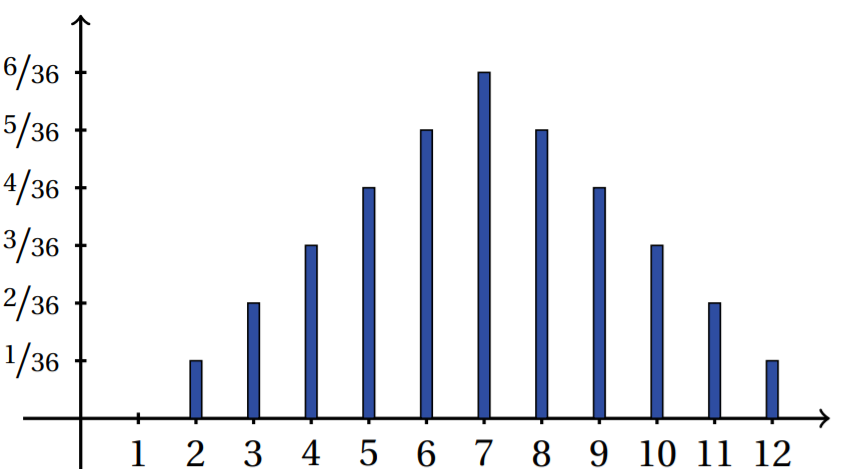
\includegraphics[width=8cm]{somme.png}
\end{center}
\end{Exemple}


\begin{Theoreme}[Construire un espace de probabilité à partir d'une loi]
Soit $(x_1,\dots,x_n)$ une famille finie de réels et $(p_1,\dots,p_n)$ une famille de réels positifs telle que $\sum_{i=1} p_i = 1$.\\
Alors il existe un
espace probabilisé $(\Omega ,\mathcal{P}(\Omega) ,P)$ et une variable aléatoire  $X$ sur cette espace et à valeurs dans  $\{x_1,\dots,x_n\}$ telle que : 
$$ \forall i \in \Intf{1}{n}:\quad  P( X = x_i ) = p_i.$$
\end{Theoreme}
\begin{Demonstration}
Soit $\Omega=\{x_1,\dots,x_n\}$ et $P$ la probabilité définie sur $(\Omega,\mathcal{P}(\Omega))$ par :
$$\forall i \in\Intf{1}{n}:\quad P(\{x_i\})=p_i.$$
Soit $X$ l'application identité. On vérifie que   $P( X = x_i )=P(\{x_i\})=p_i$, pour tout $i\in \Intf{1}{n}.$ 
\end{Demonstration}
\begin{Remarque}
Ce théorème permet de définir une variable aléatoire par sa loi de probabilité sans avoir à étudier l'expérience aléatoire sous-jacente, c'est à dire définir l'espace de probabilité $(\Omega,\mathcal{P}(\Omega),P)$ et la fonction de la variable aléatoire. Par exemple, on modélise l'expérience aléatoire d'un lancer de dé en posant : la variable aléatoire $X$ représente le chiffre du dé avec $p_1=p_2=p_3=p_4=p_5=p_6=\frac{1}{6}$.    
\end{Remarque}
\begin{DefinitionProposition}[Fonction d'une variable aléatoire]
Soit $X$ une variable aléatoire.\\
Soit $f:\R\to \R$ une application quelconque.\\
L'application \defi{$f\circ  X$}
\[ \Fonction{f\circ  X}{\Omega}{\R}{\omega}{f(X(\omega))} \]
est une variable aléatoire réelle.\\
L'usage veut qu'on la note abusivement $f(X)$ au lieu de $f\circ X$.\\
\begin{center}
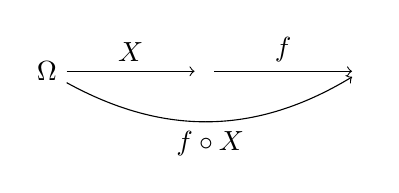
\begin{tikzpicture}[scale=1]
\node (set1) at (0,0) {$\Omega$};
\node (set2) at (2,0) {$\R$};
\node (set3) at (4,0) {$\R$};
\draw[->] (set1) -- (set2)node[midway,above]{$X$};
\draw[->] (set2) -- (set3)node[midway,above]{$f$};
\draw[->] (set1) to[bend right]node[midway,below]{$f\circ X$} (set3);
\end{tikzpicture}
\end{center}
On a $$\forall y\in f(X)(\Omega):\quad P(f(X)=y)=\sum_{x\in X(\Omega) \text{ tel que }f(x)=y }P(X=x)= \sum_{i\in\Intf{1}{n} \text{ tel que }f(x_i)=y }P(X=x_i).$$  
\end{DefinitionProposition}
\begin{Exemple}[Jeu]
Le gain obtenu est fonction de la somme obtenue avec les deux dés. La modélisation est d'appliquer une fonction à la somme, $s$, des dés  : 
 \[ \Fonction{G}{\Intf{2}{12}}{\{-1,0,2\}}{s}{\begin{cases}2&\text{ si }s=2 \text{ ou } 12\\-1&\text{ si }s=7\\0 &\text{ sinon} \end{cases}}.\]
 La variable aléatoire Gain est $G\circ X$.\\ 
Vérifions sur un exemple la modélisation. Si le jet des dés donne $\omega=(1,6)$, le gain de -1.
 On a bien $G\circ S(\omega=(1,6))=G(S(1,6))=G(1+6)=G(7)=-1$.\\
La loi de probabilité $S$ est déterminé par :
\begin{center}
\begin{tabular}{|c||c|c|c|}
\hline
$k$ & -1 &  2&0\\\hline
$P(G(S)=k)$ & $\frac{6}{36}=P(S=7)$ & $\frac{2}{36}=P(S=2)+P(S=12)$& $\frac{28}{36}=1-P(G(S)=-1)+P(G(S)=2)$  \\\hline
\end{tabular}
\end{center} 
\end{Exemple}

%


\subsection{Vecteurs aléatoires}
\begin{DefinitionProposition}[Loi conjointe]
Soit $X,Y$ deux variables aléatoires.\\
On note  $(X,Y)$ le \defi{couple de variables aléatoires} prenant ses valeurs dans $\R^2$.\\
La \defi{loi conjointe} du couple $(X,Y)$ est déterminé par  :
\begin{enumerate}
\item $X(\Omega)\times Y(\Omega)=\{x_1,\dots,x_n\}\times \{y_1,\dots,y_m\} $, les valeurs prises par le couple
\item $\forall (i,j)\in  \Intf{1}{n}\times \Intf{1}{m}:\quad P(X=x_i\cap Y=y_j).$
\end{enumerate}
On note $p_{i,j}=P(X=x_i\cap Y=y_j)$.\\
Les événements $((X=x_i)\cap (Y=y_j))_{\forall (i,j)\in \Intf{1}{n}\times \Intf{1}{m}}$ forment un système complet d'événements de $\Omega$. En particulier, on a : 
$$\sum_{i=1}^n \sum_{j=1}^mP(X=x_i\cap Y=y_j)=\sum_{i=1}^n \sum_{j=1}^m p_{i,j}=1.$$ 
\end{DefinitionProposition}
\begin{Demonstration}
Démontrons que la loi conjointe est déterminée par $$\forall (i,j)\in  \Intf{1}{n}\times \Intf{1}{m}:\quad P(X=x_i\cap Y=y_j).$$
Soit $(A,B)\subset X(\Omega)\times Y(\Omega)$. Il existe $I\subset\Intf{1}{n}$ et $J\subset\Intf{1}{m}$ tel que $A=\{x_i:i\in I\}$ et $B=\{y_j:j\in J\}$.\\ On a :
$$P((X,Y)\in (A,B))= P( X\in A\cap Y\in B )= P\left(\left(\bigcup_{i\in I} (X=x_i)\right)\cap  \left(\bigcup_{j\in J} (Y=y_j)\right)\right)=P(\bigcup_{i\in I,j\in J} (X=x_i)\cap (Y=y_j) )$$.
Comme  $(\{(X=x_i)\cap (Y=y_j)\})_{i\in I,j\in J }$ est une famille d'ensembles  disjoints. On a 
$$P((X,Y)\in (A,B))= P( X\in A\cap Y\in B )= \sum_{i\in I,j\in J}P(X=x_i\cap Y=y_j).$$   
\end{Demonstration}

\begin{Definition}[Lois marginales]
Soit $(X,Y)$ un couple de variables aléatoires.\\
La loi de $X$ appelé \defi{première loi marginale} et la loi de $Y$ \defi{second loi marginale} du couple.
\end{Definition}
\begin{Proposition}[Relations]
Soit $(X,Y)$ un couple de variables aléatoires.\\
 On a :
$$\forall i\in  \Intf{1}{n}: \quad P(X=x_i)=\sum_{j=1}^{m }P((X=x_i)\cap (Y=y_j))$$
et 
$$\forall j\in  \Intf{1}{m}: \quad P(Y=y_j)=\sum_{i=1}^{n }P((X=x_i)\cap (Y=y_j)).$$ 
\begin{center}
\begin{tabular}{|c|ccccc|c|c}
\cline{1-7}
$X\textbackslash Y$ & $y_1$ &$\dots$ & $y_j$&$\dots$&$y_m$&$P(X=x_i)$\\\cline{1-7}
$x_1$ & $p_{1,1}$ &$\dots$ & $p_{1,j}$&$\dots$&$p_{1,m}$&$P(X=x_1)$\\
$\vdots$ & $\vdots$ &  & $\vdots$& &$\vdots$&$\vdots$\\
$x_i$ & $p_{i,1}$ &$\dots$ & $p_{i,j}$&$\dots$&$p_{i,m}$&$P(X=x_i)$&$\leftarrow\sum_{k=1}^m p_{i,k}$ \\
$\vdots$ & $\vdots$ &  & $\vdots$& &$\vdots$&$\vdots$\\
$x_n$ & $p_{n,1}$ &$\dots$ & $p_{n,j}$&$\dots$&$p_{n,m}$&$P(X=x_n)$\\\cline{1-7}
$P(Y=y_j)$& $P(Y=y_1)$&$\dots$&$P(Y=y_j)$&$\dots$&$P(Y=y_m)$&1\\\cline{1-7}
      & & &$\overset{\uparrow}{\sum_{k=1}^n p_{k,j}}$ & & &\\
\end{tabular}
\end{center} 
\end{Proposition}
\begin{Demonstration}
Comme les événements $( (Y=y_j))_{\forall j\in\Intf{1}{m}}$ forment un système complet d'événements de $\Omega$, d'après la proposition \ref{prop:sce} on a 
$$\forall i\in  \Intf{1}{n}: \quad P(X=x_i)=\sum_{j=1}^{m }P((X=x_i)\cap (Y=y_j))$$ .
\end{Demonstration}


\begin{Exemple}
On tire deux nombres au hasard dans $\{-1,1\}$. On note $X$ leur somme, et $Y$ leur produit. On cherche à déterminer la loi conjointe de $(X,Y)$.\\
L'espace de probabilité est  est $(\{-1;1\}^2,\mathcal{P}(\{-1;1\}^2),P)$ avec $P$ la probabilité uniforme. Pour tout $\omega=(r,b)\in\Omega$, on a $X(r,b)=r+b$ et $Y(r,b)=r.b$. Sous forme de tableau, on a :
\begin{center}
\begin{tabular}{|c|c|c|}
\hline
$r\textbackslash b$ & -1& 1 \\\hline
-1 &-2& 0 \\\hline
1 & 0& 2 \\\hline
\multicolumn{3}{c}{Définition de $X$}
\end{tabular}
\end{center}  
 \begin{center}
\begin{tabular}{|c|c|c|}
\hline
$r\textbackslash b$ & -1& 1 \\\hline
-1 &1& -1 \\\hline
1 & -1&1 \\\hline
\multicolumn{3}{c}{Définition de $Y$}
\end{tabular}
\end{center}  
$X$ prend ses valeurs dans $\{-2,0,2\}$ et $Y$ dans $\{-1,1\}$.\\
 Les variables aléatoires étant finies, il suffit de déterminer toutes les probabilités $P(X=x\text{  et }Y=y$) pour tout couple $(x,y)\in \{-2,0,2\}\times\{-1,1\}$. On a :
 \begin{itemize}
 \item $P(X=2, Y=1)=P( \{(1,1)\})\overbrace{=}^{\text{equiprobabilité}} \frac{1}{4}.$
 \item $P(X=2, Y=-1)=P( \emptyset)= 0.$
\item  $P(X=0, Y=1)=P( \emptyset)= 0.$
\item  $P(X=0, Y=-1)=P( \{(1,-1),(-1,1)\})=\frac{2}{4}=\frac 1 2.$
\item $P(X=-2, Y=1)=P( \{(-1,-1)\})=\frac{1}{4}.$
\item $P(X=-2, Y=-1)=P( \emptyset)= 0.$
 \end{itemize}
La loi de probabilité conjointe $(X,Y)$ est donc déterminée par :
\begin{center}
\begin{tabular}{|c|c|c|c|}
\hline
$X\textbackslash Y$ & -1& 1 & $P(X=x)$\\\hline
-2 & 0& 1/4 & 1/4\\\hline
0 & 1/2 &0 & 1/2\\\hline
2 & 0& 1/4 & 1/4\\\hline
$P(Y=y)$&1/2&1/2&1 \\\hline
\end{tabular}
\end{center} 
\end{Exemple}
\begin{Exemple}
Dans une classe, la répartition en fonction de l'age et du genre est :
\begin{center}
\begin{tabular}{|c|c|c|c|}
\hline
Age$\textbackslash$ Genre & Fille& Garçon & Total\\\hline
18 & 5 & 10& 15 \\\hline
19 & 2 & 6& 8 \\\hline
20 & 0 & 1 & 1 \\\hline
Total&7&17&24 \\\hline
\end{tabular}
\end{center}
On tire au hasard un élève dans la classe.\\
$X$ représente l'age de l'élève.\\
$Y$ représente le genre de l'élève avec la label 0 pour une fille et le label 1 pour un garçon.\\
La loi de probabilité conjointe $(X,Y)$ est déterminée par :
 \begin{center}
\begin{tabular}{|c|c|c|c|}
\hline
$X\textbackslash Y$ & 0& 1 & $P(X=x)$\\\hline
18 & 5/24& 10/24 & 15/24\\\hline
19 & 2/24& 6/24 & 8/24\\\hline
20 & 0/24& 1/24 & 1/24\\\hline
$P(Y=y)$&7/24&17/24&1 \\\hline
\end{tabular}
\end{center} 

\end{Exemple}

%% -----------------------------------------------------------------------------
\subsection{Indépendance et lois conditionnelles}
\begin{DefinitionProposition}[Lois conditionnelles]
Soit $(X,Y)$ un couple de variables aléatoires.\\
\begin{enumerate}
\item On appelle \defi{loi conditionnelle} de $X$ sachant $(Y = y_j )$ pour $P(Y = y_j )\neq 0$, la probabilité définie par  :
$$\forall i\in \Intf{1}{n}:\quad  P_{Y=y_j}(X=x_i)=\frac{P(X=x_i\cap Y=y_j) } {P(Y=y_i)}$$ 
\item On appelle \defi{loi conditionnelle} de $Y$ sachant $(X = x_i )$ pour $P(X = x_i )\neq 0$, la probabilité définie par  :
$$\forall j\in \Intf{1}{m}:\quad  P_{X=x_i}(Y=y_j)=\frac{P(X=x_i\cap Y=y_j) } {P(X=x_i)}$$ 
\end{enumerate}
\end{DefinitionProposition}

\begin{Remarque}
Les lois marginales et les lois conditionnelles déterminent la loi conjointe :
$$\forall (i,j)\in  \Intf{1}{n}\times \Intf{1}{m}:\quad P(X=x_i\cap Y=y_j)=P_{X=x_i}(Y=y_j)P(X=x_i)$$
$$\forall (i,j)\in  \Intf{1}{n}\times \Intf{1}{m}:\quad P(X=x_i\cap Y=y_j)=P_{Y=y_j}(X=x_i)P(Y=y_j)$$
\end{Remarque}
\begin{Definition}[Indépendance]
Soit $(X,Y)$ un couple de variables aléatoires.\\
On dit que $X$ et $Y$ sont \defi{indépendantes} si 
$$ \forall (i,j)\in  \Intf{1}{n}\times \Intf{1}{m}:\quad P( (X=x_i)\cap (Y=y_j) ) = P(X=x_i) P(Y=y_j).$$
\end{Definition}
\begin{Remarque} Dans la modélisation d'une expérience aléatoire, l'hypothèse d'indépendance des variables aléatoires est souvent une donnée de l'expérience et 
non pas une propriété à vérifier. Par exemple, la modélisation de l'expérience du jeter de deux dés serait :
\begin{itemize}
\item $X_1$,  la variable aléatoire représentant le chiffre du premier dé,
\item $X_2$, la variable aléatoire représentant le chiffre du second dé,
\item $X_1$ et $X_2$, supposées indépendantes,
\item $S=X_1+X_2$, la somme des deux dés.
\end{itemize}
\end{Remarque}
\begin{Theoreme}
Soit $(X,Y)$ un couple de variables aléatoires.\\
Si $X$ et $Y$ sont indépendantes, il en va de même pour les variables aléatoires $f(X)$ et $g(Y)$
où $f:\R\to \R$ et $g:\R\to \R $ sont deux applications quelconques.
\end{Theoreme}




%% -----------------------------------------------------------------------------
\subsection{Espérance}
L'espérance mathématique d'une variable aléatoire réelle est la moyenne pondérée par les probabilités d'apparition de chaque valeur. Le théorème de la loi forte des grands nombres démontrera que l'espérance est la valeur que l'on s'attend à trouver, en moyenne, si l'on répète un grand nombre de fois la même expérience aléatoire.
\begin{Definition}[Espérance d'une variable aléatoire]
Soit $X$ une variable aléatoire.\\
L'\defi{espérance} de $X$ est
\[ E(X) = \sum_{\forall i\in  \Intf{1}{n} } x_i P(X=x_i) \]
\end{Definition} 
\begin{Exemple}[Somme de deux dés]
Reprenons l'exemple du lancer de deux dés en notant $S$ la somme des chiffres obtenus. 
L'espérance de $S$ vaut alors :
$$E(S ) = \sum_{s\in S (\Omega)} sP(S = s)=  2.\frac{1}{36}+3.\frac{2}{36}+4.\frac{3}{36}+5.\frac{4}{36}+6.\frac{5}{36}+7.\frac{6}{36}+8.\frac{5}{36}+9.\frac{4}{36}+10.\frac{3}{36}+11.\frac{2}{36}+12.\frac{1}{36}=7.$$
\end{Exemple}


\begin{Theoreme}[Formule de transfert]
Soit $X$ une variable aléatoire et  $f:\R\to \R$.\\
On a
\[ E(f(X)) =  \sum_{\forall i\in  \Intf{1}{n} }  f(x_i) P(X=x_i). \]
\end{Theoreme}
\begin{Demonstration}
$$ E(f(X)) = \sum_{\forall j\in  \Intf{1}{m }}  y_j P(f(X)=y_i)= \sum_{\forall j\in  \Intf{1}{m }}  y_j  \sum_{\forall i\in\Intf{1}{n} :f(x_i)=y_j }P(X=x_i)= \sum_{\forall j\in  \Intf{1}{m }}    \sum_{\forall i\in\Intf{1}{n} :f(x_i)=y_j }y_j P(X=x_i).$$ 
D'où
$$ E(f(X)) = \sum_{\forall j\in  \Intf{1}{m }}    \sum_{\forall i\in\Intf{1}{n}:f(x_i)=y_j }f(x_i) P(X=x_i)=\sum_{\forall i\in\Intf{1}{n} }f(x_i) P(X=x_i).$$ 
\end{Demonstration}

\begin{Remarque}
La formule de transfert permet de  calculer $E(f(X))$ sans avoir à déterminer la loi de $f(X)$.\\
Dans l'exemple du jeu, l'espérance de la variable aléatoire $G(X)$ représente le gain  moyen du joueur. On applique la formule du transfert :
\[E(G(S))=\sum_{s\in \{2,3,\dots,12\}}  G(s) P(S=s)=2P(S=2)-1P(S=7)+2P(S=12)=2\frac{1}{36}-1\frac{6}{36}+2\frac{2}{36}=-\frac{1}{18}.\]
En conclusion, ce jeu n'est pas favorable au joueur.
\end{Remarque}


\begin{Theoreme}[Espérance du produit de variables aléatoires]
Soit $X$ et $Y$ deux variables aléatoires indépendantes.\\
Alors \[ E(XY) = E(X) E(Y). \]
\end{Theoreme}
\begin{Demonstration}
On applique le théorème de transfert à la variable aléatoire $f(X,Y)=XY$ d'où
$$\begin{aligned}
 E(XY) &= \sum_{ \forall (i,j)\in  \Intf{1}{n}\times \Intf{1}{m}} x_i y_j P(X=x_i\cap Y=y_j )\\
       &\overbrace{=}^{\text{indépendance} } \sum_{  \forall (i,j)\in  \Intf{1}{n}\times \Intf{1}{m}} x_i y_j P(X=x_i) P(Y=y_j)\\
       &= \sum_{ i=0 }^n  \sum_{j=0}^m  x_i y_j P(X=x_i) P(Y=y_j)\\
       &= \sum_{ i=0 }^n  x_i P(X=x_i) \sum_{j=0}^m y_j  P(Y=y_j) \\
       &= E(X)E(Y).
\end{aligned}$$ 
\end{Demonstration}


\begin{Proposition}[Propriétés de l'espérance]
Soit $X$ et $Y$ deux variables aléatoires réelles et $(a,b)\in\R^2$.
\begin{itemize}
\item
  $E(a) = a$.
\item
 \textit{linéarité} :  $E(aX+bY) = aE(X)+bE(Y)$.
\item
  Si $P(X\geq 0)=1$, alors $E(X)\geq 0$.
\item
  Si $P(X\leq Y)=1$, alors $E(X)\leq E(Y)$.
\end{itemize}
\end{Proposition}

\begin{Definition}[Centrée]
Une variable aléatoire est dite \defi{centrée} si son espérance est nulle.
\end{Definition}
\begin{Exemple}[Centrer une variable aléatoire]
Soit $X$ une variable aléatoire.\\
La variable aléatoire $Y=X-E(X)$ est centrée car $E(Y)=E(X-E(X))=E(X)-E(E(X))=E(X)-E(X)=0$
\end{Exemple}
\begin{Demonstration}
\begin{itemize}
\item Dans l'expression $E(a)$,  $a$ est la variable aléatoire  définie par $\omega\mapsto a$  d'où $E(a )=\overbrace{a}^{\in\R}P(a=\overbrace{a}^{\in\R})=\overbrace{a}^{\in\R}.$\\
\item On applique le théorème de transfert à la variable aléatoire $f(X,Y)=aX+bY$ d'où
$$\begin{aligned}
 E(aX+bY) &= \sum_{ \forall i\in  \Intf{1}{n}}\sum_{ \forall j\in  \Intf{1}{m}} (ax_i+b y_j) P(X=x_i\cap Y=y_j )\\
       &=  a\sum_{ \forall i\in  \Intf{1}{n}}x_i\sum_{ \forall j\in  \Intf{1}{m}} P(X=x_i\cap Y=y_j )+b\sum_{ \forall j\in  \Intf{1}{m}} y_j \sum_{ \forall i\in  \Intf{1}{n}}P(X=x_i\cap Y=y_j )
 \\
       &=  a\sum_{ \forall i\in  \Intf{1}{n}}x_i P(X=x_i )+b\sum_{ \forall j\in  \Intf{1}{m}}  y_jP( Y=y_j )\\
       &=  aE(X)+bE(Y).
\end{aligned}$$
\item  Soit $X$ une variable aléatoire telle que $P(X\geq 0)=1$ d'où $P(X< 0)=0$.\\
De plus, pour tout $x\in \R$, $P(X=x)=0$ car $\{X=x\}\subset \{X< 0\}$.\\
\[ E(X) = \sum_{\forall i\in  \Intf{1}{n} } x_i P(X=x_i)= \sum_{\forall i\in  \Intf{1}{n}: x_i\geq 0 } x_i P(X=x_i)\geq 0.\]
\item Soit $X$ une variable aléatoire telle que $P(Y- X\leq 0)=1$. Ainsi $E(Y- X)\geq 0$ et $E(X)\leq E(Y)$.
\end{itemize}
\end{Demonstration}
%


\subsection{Variance}
La variance est une mesure de la dispersion des valeurs d'une loi de probabilité.
\begin{Definition}[variance d'une variable aléatoire]
Soit $X$ une variable aléatoire.\\
La \defi{variance} de $X$ est $$E\left( (X-E(X))^2\right)$$ et on la note $V(X)$.\\
L'\defi{écart-type} est $\sigma(X) =\sqrt{V(X)}$.
\end{Definition}
\begin{Proposition}[Formule de K\oe nig-Hugens]
Soit $X$ une variable aléatoire.\\
Pour tout $a>0$, on a :
\[ V(X) = E(X^2)-(E(X))^2 \]
\end{Proposition}
\begin{Demonstration}
$$\begin{aligned}
  V(X) &= E\left( (X-E(X))^2\right) \\
  V(X) &= E\left( X^2-2E(X)X + E(X)^2\right)\\
  V(X) &= E(X^2)-2E(X)E(X) + E(X)^2 \text{ car } E \text{ linéaire et }E(a)=a\\
  V(X) &= E(X^2)-(E(X))^2
\end{aligned}$$
\end{Demonstration}




\begin{Exemple}[Somme de deux dés]
Reprenons l'exemple du lancer de deux dés en notant $S$ la somme des chiffres obtenus. 
On a :
$$E(S^2 )\overbrace{=}^{\text{th transfert}} \sum_{s\in S (\Omega)} s^2P(S = s)=  2^2.\frac{1}{36}+3^2.\frac{2}{36}+4^2.\frac{3}{36}+\dots+12^2.\frac{1}{36}=\frac{329}{6}.$$
La variance de $S$ vaut alors :
$$V(S)=E(S^2 )-(E(S))^2=\frac{329}{6}-7^2=\frac{35}{6}.$$
et son écart-type
$$\sigma(S)=\sqrt{V(S)}\approx 2,42.$$
\end{Exemple}
\begin{Definition}[Réduite]
Une variable aléatoire est dite \defi{réduite} si sa variance est égale à .
\end{Definition}
\begin{Exemple}[Centrer et réduire une variable aléatoire]
Soit $X$ une variable aléatoire.\\
La variable aléatoire $Y=\frac{X-E(X)}{\sigma(X)}$ est centrée réduite.
\end{Exemple}

\begin{Definition}[Covariance de deux variables aléatoires]
Soit $X$ et $Y$ deux variables aléatoires.\\
La \defi{covariance} de $X$ et $Y$ est $$E( (X-E(X)) (Y-E(Y)) )$$ et on la note $\mathrm{Cov}(X,Y)$.
\end{Definition}
\begin{Proposition}[Propriétés]
Soit $X$ et $Y$ deux variables aléatoires.
\begin{itemize}
\item
  $V(aX+b) =E\left( (X-E(X))^2\right)$.
  \item
  $Var(X+Y) = Var(X) + Var(Y) + 2\mathrm{Cov}(X,Y)$.
\item
  Si $X$ et $Y$ sont indépendantes, alors $V(X+Y) =V(X)+V(Y)$.
\end{itemize}
\end{Proposition}
\begin{Demonstration}
\begin{itemize}
\item
  $V(aX+b) =E( (aX+b-E(aX+b))^2)=E( a^2(X-E(X))^2)=a^2V(X)$ car $E$ linéaire..
\item
   $V(X+Y) =E( (X+Y-E(X+Y))^2)= E( (X-E(X))^2) +  E( (Y-E(Y))^2)+2E( (X-E(X)(Y-E(Y))) =Var(X) + Var(Y) + 2\mathrm{Cov}(X,Y)$.
\item
Si $X$ et $Y$ sont indépendantes, alors $X-E(X)$ et $Y-E(Y)$ sont indépendantes, d'où $$E( (X-E(X)(Y-E(Y)))=E(X-E(X)) E(Y-E(Y))=0.$$
\end{itemize}
\end{Demonstration}


\begin{Definition}[Corrélation]
Soit $X$ et $Y$ deux variables aléatoires de variance non nulles.\\
Le \defi{coefficient de corrélation} de $X$ et $Y$ est
\[ \rho(X,Y) = \frac{\mathrm{Cov}(X,Y)}{\sigma(X)\sigma(Y)} \]
\end{Definition}
\begin{Proposition}[Propriétés]
Soit $X$ et $Y$ deux variables aléatoires de variance non nulles.
\begin{itemize}
\item
  $\rho(X,Y) \in [-1,1]$
\item
  $\rho(X,Y) = ±1$ si et seulement si il existe deux réels $a$ et $b$ tels que l'événement $\{Y=aX+b\}$ soit certain.
\item
  Si $X$ et $Y$ sont indépendantes, alors $\rho(X,Y) = 0$. On dit qu'elles sont décorrélées.
  La réciproque est fausse.
\end{itemize}
\end{Proposition}
\begin{Demonstration}
On utilise l'inégalité de Cauchy-Schwarz $|\mathrm{Cov}(X, Y )| \leq \sigma (X)\sigma (Y )$ (voir un cours d'algèbre bilinéaire pour la preuve de cette inégalité).
\end{Demonstration}
%% -----------------------------------------------------------------------------
\subsection{Lois usuelles}

\subsubsection{Loi uniforme}

Lorsque on se trouve dans une situation d'équiprobabilité par exemples "jeter un dé équilibré", " tirer une boule dans une urne de boules distinctes", "choisir un élève au hasard pour passer au tableau", on modélise l'expérience aléatoire avec une variable aléatoire suivant une loi uniforme.
\begin{DefinitionProposition}[Loi uniforme]
Une variable aléatoire $X$ suit la \defi{loi uniforme} sur $\Intf{1}{n}$
si 
\begin{enumerate}
\item $X(\Omega)=\Intf{1}{n}$,
\item $\forall i\in \Intf{1}{n}:\quad  P(X=i) = \frac{1}{n}.$ 
\end{enumerate} 
On note $X \hookrightarrow \mathcal{U}(E)$.\\
On a : $E(X)=\frac{n+1}{2}$ et $V(X)=\frac{n^2-1}{2}$.
\end{DefinitionProposition}
\begin{Demonstration}
L'espérance est :
$$E(X)=\sum_{i=1}^n iP(X=i)=\sum_{i=1}^n i \frac{1}{n}=\frac{1}{n} \sum_{i=1}^n i =\frac{1}{n} \frac{n(n+1)}{2}=\frac{n+1}{2}.$$
Pour la variance, on a :
$$E(X^2)=\sum_{i=1}^n i^2P(X=i)=\frac{1}{n} \sum_{i=1}^n i^2 =\frac{1}{n} \frac{(2n+1)n(n+1)}{6}=\frac{(2n+1)(n+1)}{6}.$$
Ainsi, on a :
$$V(X)=E(X^2) - (E(X))^2=\frac{(2n+1)(n+1)}{6}- \left(\frac{n+1}{2}\right)^2=\frac{n+1}{2}\left(\frac{2(2n+1)-3(n+1)}{3}\right),$$
$$V(X)=\frac{n+1}{2}\frac{n-1}{6}=\frac{n^2-1}{12}.$$
\end{Demonstration}
\subsubsection{Loi de Bernoulli}
Lorsque l'issue est binaire du
type "succès ou échec", "vrai ou faux", "marche ou arrêt", pile
ou face", etc, on modélise l'expérience aléatoire avec une variable aléatoire suivant une loi de Bernoulli.

\begin{DefinitionProposition}[Loi de Bernoulli]
Une variable aléatoire $X$ suit la \defi{loi de Bernoulli} de paramètre $p$
si 
\begin{enumerate}
\item $X(\Omega)=\{0,1\}$,
\item $P(X=1) = p \quad \text{et} \quad P(X=0) = 1-p.$ 
\end{enumerate} 
On note $X \hookrightarrow  \mathcal{B}(p)$.\\
On a : $E(X)=p$ et $V(X)=p(1-p)$.
\end{DefinitionProposition}
\begin{Demonstration}
L'espérance est :
$$E(X)=0 P(X=0)+1P(X=1)=p.$$
Pour la variance, on a :
$$E(X^2)=0^2P(X=0)+1^2P(X=1)=p^2.$$
Ainsi, on a :
$$V(X)=p-p^2=p(1-p).$$
\end{Demonstration}

\begin{DefinitionProposition}[Loi indicatrice]
Soit $A$ est un événement de $\Omega$.\\
 La variable aléatoire réelle $1_A$ définie par  
$$1_A(\omega) =\begin{cases}1\text{ si }\omega \in A\\0\text{ si }\omega \in \bar A \end{cases}$$
est une variable de Bernoulli de paramètre $p=P(A)$. On l'appelle \defi{loi indicatrice} de l'événement $A$.
\end{DefinitionProposition}

\subsubsection{Loi Binomiale}
Lorsque on répète $n$ fois une expérience de Bernoulli indépendamment  des unes et des
autres et que l'on compte le nombre de succès, par exemples "nombre de faces obtenus après n lancers", on modélise l'expérience aléatoire avec une variable aléatoire suivant une loi binomiale.\\
En effet, soit $X_1, X_2,\dots, X_n$ $n$ variables aléatoires indépendantes de loi de Bernoulli de même paramètre $p$.\\
On pose $X=X_1+ X_2+\dots+ X_n$ la variable aléatoire représentant le nombre de succès.\\
On a $X(\Omega) = \Intf{0}{n}$ et

$$(X = k) = (X_1+ X_2+\dots+ X_n=k)=\bigcup_{I\subset\Intf{1}{n}:\operatorname{Card} (I)=k} \left(\cap_{i\in I} (X_i=1)\right)\cap \left(\cap_{i\in \Intf{1}{n}\setminus I} (X_i=0)\right)$$
Comme l'union est disjointe, on a :
$$P(X = k) =\sum_{I\subset\Intf{1}{n}:\operatorname{Card} (I)=k } P(\left(\cap_{i\in I} (X_i=1)\right)\cap \left(\cap_{i\in \Intf{1}{n}\setminus I} (X_i=0)\right))$$
Comme les variables aléatoires sont indépendantes, on a :
$$P(X = k) =\sum_{I\subset\Intf{1}{n}:\operatorname{Card} (I)=k} p^k(1-p)^{n-k}$$
Le nombre de parties à $k$ éléments de l'ensemble $\Intf{1}{n}$ est le coefficient binomial correspondant à la position des $k$ succès, d'où
$$P(X = k) =\begin{pmatrix}n\\k\end{pmatrix} p^k(1-p)^{n-k},$$
où $p^k$ est la probabilité d'obtention de ces $k$
succès et $(1 - p)^{n-k}$ est la probabilité d'obtention des échecs.\\
On définit donc :
\begin{Definition}[Loi binomiale]
Une variable aléatoire $X$ suit la \defi{loi binomiale} de paramètres $n$ et $p$
si
\begin{enumerate}
\item $X(\Omega)= \Intf{1}{n}$,
\item $\forall i\in\Intf{1}{n}:\quad\ P(X=i) = \binom{n}{i} p^i (1-p)^{n-i}.$ 
\end{enumerate} 
On note $X \hookrightarrow  \mathcal{B}(n,p)$.\\
On a : $E(X)=np$ et $V(X)=np(1-p)$.
\end{Definition}
\begin{Proposition}[Loi des tirages avec remise]
Soit $X_1, X_2,\dots, X_n$ $n$ variables aléatoires indépendantes de loi de Bernoulli de même paramètre $p$.\\
Alors $X=X_1+ X_2+\dots+ X_n$ suit une loi binomiale de paramètres $n, p$.\\
En d'autres termes, si l'expérience aléatoire est  une répétition de $n$ épreuves identiques et indépendantes tel que chaque épreuve est une expérience Bernouilli de paramètre  $p$ et si $S$ est égale au nombre de succès des $n$ épreuves de l'expérience, alors $S$  suit une loi binomiale de paramètres $n, p$.\\
Inversement, si $X$ suit une loi binomiale de paramètres $n, p$, alors il existe $X_1, X_2,\dots, X_n$ $n$ variables aléatoires indépendantes de loi de Bernoulli de même paramètre $p$ tel que $X=X_1+ X_2+\dots+ X_n$.    
\end{Proposition}
\begin{Demonstration}
La preuve a été faite dans l'introduction de la loi binomiale.
\end{Demonstration}
\begin{Remarque}
Pour $n=1$, on retrouve la loi de Bernoulli de paramètre $p$.
\end{Remarque}
\begin{Proposition}[Espérance et Variance]
Soit $X\hookrightarrow  \mathcal{B}(n,p)$.\\
On a : $E(X)=np$ et $V(X)=np(1-p)$.
\end{Proposition}
\begin{Demonstration}
Au lieu d'un calcul directe de l'espérance $E(X)=\sum_{i=0}^n i   \binom{n}{i} p^i (1-p)^{n-i} p^i (1-p)^{n-i}$, nous utilisons la proposition sur la loi des tirages avec remise.\\
Il existe $X_1, X_2,\dots, X_n$ $n$ variables aléatoires indépendantes de loi de Bernoulli de même paramètre $p$ tel que $X=X_1+ X_2+\dots+ X_n$. Ainsi :
$$E(X)=E(X_1+ X_2+\dots+ X_n)\overbrace{=}^{\text{linéarité}}E(X_1)+ E(X_2)+\dots+ E(X_n)=np.$$
Aussi, la variance est égale à :
$$V(X)=V(X_1+ X_2+\dots+ X_n)\overbrace{=}^{\text{indépendantes}}V(X_1)+ V(X_2)+\dots+ V(X_n)=np(1-p).$$
\end{Demonstration}


\subsection{Convergence et approximations}

%\begin{Proposition}[Approximation d'une loi binomiale par une loi de Poisson]
%Soit $(X_n)_{n\in\N}$ une suite de variables aléatoires tel que $X_n\hookrightarrow \mathcal{B}(n,p_n)$ et $\lim\limits_{n\to\infty}np_n=\lambda$.\\
%Alors on a :
%$$\forall k \in \N:\quad  \lim\limits_{n\to\infty} P(X_n = k) = e^{-\lambda}\frac{\lambda^k}{k!}.$$
%\end{Proposition}
%\begin{Demonstration}
%Soit $k\in \N$. On a :
%$$\begin{aligned}
%P(X_n = k) &= \begin{pmatrix}n \\ k \end{pmatrix} (p_n)^k (1-p_n)^{n-k}\\
%&= \frac{1}{k!} n.(n-1).\dots (n-k+1)(p_n)^k (1-p_n)^{n-k} \\
%&= \frac{1}{k!} 1.(1-1/n).\dots (1-(k+1)/n)(p_n/n)^k (1-p_n)^{n-k} \\
%\end{aligned}$$
%D'une part  $\overbrace{1.(1-1/n).\dots (1-(k+1)/n)}^{k \text{ facteurs fixes}}\tend[n\to+\infty]1$, d'autre part $(p_n/n)^k\tend[n\to+\infty] \lambda^k$ et enfin $(1-p_n)^{n-k}=e^{(n-k)\ln(1-p_n)}\tend[n\to+\infty] e^{-\lambda}$ car $(n-k)\ln(1-p_n)\equivalent[n\to+\infty] -np_n$. Finalement
%$$\lim\limits_{n\to\infty} P(X_n = k) = e^{-\lambda}\frac{\lambda^k}{k!}.$$
%\end{Demonstration}
%%TODO DEMO
%
%%TODO loi faible des grands nombres
%% Rajouter 
%En pratique, si $X$ est une variable aléatoire suivant la loi binomiale $\mathcal{B}(n,p)$ avec $n\geq 30$, $p\leq 0,10$ et $np\geq 15$, on peut approximer la loi de $X$ par la loi de Poisson de paramètre $np$.\\
%Ce théorème  justifie le fait que la loi de Poisson est utilisée comme modèle de certaines expériences aléatoires (nombre de clients entrant dans un magasin, nombre de coquilles dans une page de journal,...).

\begin{Proposition}[Inégalité de Markov]
Soit $X$ une variable aléatoire réelle positive.\\
Pour tout $a > 0$, on a :
\[ P(X\geq a) \leq \frac{E(X)}{a}.\]
\end{Proposition}
\begin{Proposition}[Inégalité de Bienaymé-Tchebychev]
Soit $X$ une variable aléatoire réelle.
Pour tout $a>0$, on a
\[ P( |X-E(X)| \geq a ) \leq \frac{V(X)}{a^2} \]
\end{Proposition}
%TODO FAIRE LES DEMOS
Cette inégalité présente un intérêt théorique en majorant la
probabilité qu'une variable aléatoire s'écarte de sa moyenne. Nous allons l'utiliser pour prouver la loi faible des grands
nombres.

Lors d'un lancer d'une pièce de monnaie équilibrée, les deux côtés « pile » et « face » apparaissent de façon équiprobable pour des raisons de symétrie : on ne s'attend pas plus à l'un ou à l'autre côté. Cette mesure de l'attente s'appuie souvent sur une considération statistique : on observe que la fréquence des occurrences de chaque côté se rapproche de 1/2. 
\begin{center}
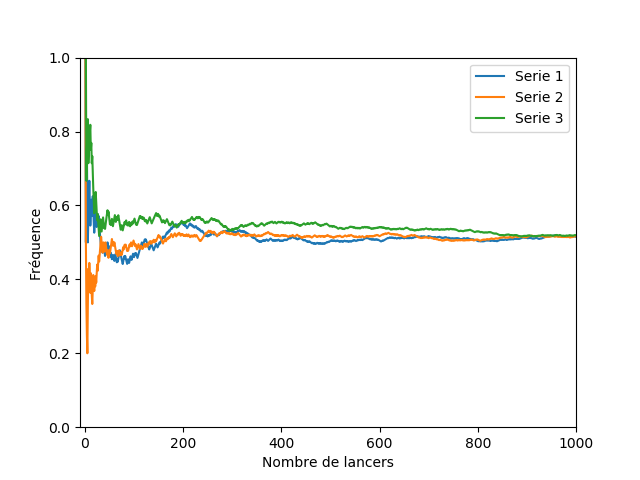
\includegraphics[width=12cm]{frequence_lancer.png}
\end{center}
Le théorème de la loi des grands nombres permet de justifier ce résultat en interprétant la probabilité comme une fréquence de réalisation.\\
La modélisation de cette expérience aléatoire est :
\begin{enumerate}
\item  \impo{n\up{ième} lancer} :  pour tout $i\in\N^*$,  la variable aléatoire $X_i$, représente le résultat du n\up{ième} lancer. Elle  suit une loi Bernoulli de paramètre $p$ (l'issue 0 représente le pile et l'issue 1 le face). Elles sont supposées indépendantes.  On a $E(X_i) = (1 - p).0 + p.1  = p.$ 
\item \impo{fréquence} : pour tout $n\in\N^*$,  la variable aléatoire $S_n$, représente la moyenne des résultats obtenus au cours des n premiers lancers, soit :
$$ S_n =\frac{X_1+X_2+\dots+X_n}{n}$$ 
\end{enumerate}
L'issue, $\omega$, correspondant à une succession de faces, $X_n(\omega)=1$ pour tout $n\in \N^*$, existe. Donc $1$ est une valeur possible de la variable aléatoire $S_n$. Cependant, le théorème de la loi faible des grands nombres prouve que la \impo{probabilité} que $S_n$ s'écarte de l'espérance $E(X_n)$ tend vers 0 quand $n$ tend vers l'infini. 
\begin{Theoreme}[Loi faible des grands nombres]
Soit $(X_n)_{n\in\N^*}$ une suite de variables aléatoires indépendantes et de même loi, admettant une espérance $m$ et un écart
type $\sigma$.\\
On pose $S_n =\frac{X_1+X_2+\dots+X_n}{n}.$\\
Alors 
$$ \forall \epsilon>0: \quad P\left(\left| S_n - m \right|\geq \epsilon \right )\xrightarrow[n\to+\infty]{}0.$$
On dit que la suite des variables aléatoires $(s_n)$ \defi{converge en probabilité} vers $m$. 
\end{Theoreme}
\begin{Demonstration}
D'après l'inégalité de Bienaymé-Tchebychev et par indépendance des variables aléatoires,
$$ \forall \epsilon>0: \quad P\left(\left| S_n - m \right|\geq \epsilon\right)\leq \frac{V(S_n)}{\epsilon^2}=\frac{\frac{V(X_1+X_2+\dots+X_n)}{n^2}}{\epsilon^2}=\frac{\sigma^2}{n\epsilon^2} \xrightarrow[n\to+\infty]{}0.$$
\end{Demonstration}


\begin{Theoreme}[Théorème de Bernoulli]
Soit $(A_n)_{n\in\N}$ une suite 
d'événements indépendants de même probabilité $p$.\\
La suite des  
variables aléatoires $\frac 1 n \sum_{i=0}^N 1_{A_i}$ converge en probabilité vers $p$. 
\end{Theoreme}
\begin{Demonstration} Les variables aléatoires $1_{A_n}$ sont  
indépendantes de même loi de Bernoulli. D'après la loi faible des grands nombres, la suite  des  
variables aléatoires $\frac 1 n \sum_{i=0}^N 1_{A_i}$ converge en probabilité vers $E(X_1)=p$.
\end{Demonstration}
\begin{Remarque}
Ce théorème assure qu'en répétant une expérience aléatoire, la fréquence 
des occurrences d'un événement converge en probabilité  
vers la probabilité de l'événement.
Ce théorème apporte la cohérence entre l'approche de la modélisation probabiliste et  
l'approche fréquentiste.\\
Le TP Python \url{https://github.com/VincentTariel/cours/blob/master/probabilite/simulation_variable_aleatoire_avtivite_python.pdf} permet de vous familiariser sur les applications de ce théorème.
\end{Remarque}



\end{document}
